\documentclass[11pt,compress,t,notes=noshow, xcolor=table]{beamer}


% graphicx and color are loaded via lmu-lecture.sty
% maxwidth is the original width if it is less than linewidth
% otherwise use linewidth (to make sure the graphics do not exceed the margin)
% TODO: Remove once cleared to be superfluous
% \makeatletter
% \def\maxwidth{ %
%   \ifdim\Gin@nat@width>\linewidth
%     \linewidth
%   \else
%     \Gin@nat@width
%   \fi
% }
% \makeatother

% ---------------------------------%
% latex-math dependencies, do not remove:
% - mathtools
% - bm
% - siunitx
% - dsfont
% - xspace
% ---------------------------------%

%--------------------------------------------------------%
%       Language, encoding, typography
%--------------------------------------------------------%

\usepackage[english]{babel}
\usepackage[utf8]{inputenc} % Enables inputting UTF-8 symbols
% Standard AMS suite (loaded via lmu-lecture.sty)

% Font for double-stroke / blackboard letters for sets of numbers (N, R, ...)
% Distribution name is "doublestroke"
% According to https://mirror.physik.tu-berlin.de/pub/CTAN/fonts/doublestroke/dsdoc.pdf
% the "bbm" package does a similar thing and may be superfluous.
% Required for latex-math
\usepackage{dsfont}

% bbm – "Blackboard-style" cm fonts (https://www.ctan.org/pkg/bbm)
% Used to be in common.tex, loaded directly after this file
% Maybe superfluous given dsfont is loaded
% TODO: Check if really unused?
% \usepackage{bbm}

% bm – Access bold symbols in maths mode - https://ctan.org/pkg/bm
% Required for latex-math, preferred over \boldsymbol
% https://tex.stackexchange.com/questions/3238/bm-package-versus-boldsymbol
\usepackage{bm}

% pifont – Access to PostScript standard Symbol and Dingbats fonts
% Used for \newcommand{\xmark}{\ding{55}, which is never used
% aside from lecture_advml/attic/xx-automl/slides.Rnw
% \usepackage{pifont}

% Quotes (inline and display), provdes \enquote
% https://ctan.org/pkg/csquotes
\usepackage{csquotes}

% Adds arg to enumerate env, technically superseded by enumitem according
% to https://ctan.org/pkg/enumerate
% Replace with https://ctan.org/pkg/enumitem ?
% Even better: enumitem is not really compatible with beamer and breaks all sorts of things
% particularly the enumerate environment. The enumerate package also just isn't required
% from what I can tell so... don't re-add it I guess?
% \usepackage{enumerate}

% Line spacing - provides \singlespacing \doublespacing \onehalfspacing
% https://ctan.org/pkg/setspace
% \usepackage{setspace}

% mathtools – Mathematical tools to use with amsmath
% https://ctan.org/pkg/mathtools?lang=en
% latex-math dependency according to latex-math repo
\usepackage{mathtools}

% Maybe not great to use this https://tex.stackexchange.com/a/197/19093
% Use align instead -- TODO: Global search & replace to check, eqnarray is used a lot
% $ rg -f -u "\begin{eqnarray" -l | grep -v attic | awk -F '/' '{print $1}' | sort | uniq -c
%   13 lecture_advml
%   14 lecture_i2ml
%    2 lecture_iml
%   27 lecture_optimization
%   45 lecture_sl
\usepackage{eqnarray}
% For shaded regions / boxes
% Used sometimes in optim
% https://www.ctan.org/pkg/framed
\usepackage{framed}

%--------------------------------------------------------%
%       Cite button (version 2024-05)
%--------------------------------------------------------%

% Superseded by style/ref-buttons.sty, kept just in case these don't work out somehow.

% Note this requires biber to be in $PATH when running,
% telltale error in log would be e.g. Package biblatex Info: ... file 'authoryear.dbx' not found
% aside from obvious "biber: command not found" or similar.
% Tried moving this to lmu-lecture.sty but had issues I didn't quite understood,
% so it's here for now.

\usepackage{hyperref}

% Only try adding a references file if it exists, otherwise
% this would compile error when references.bib is not found
% NOTE: Bibliography packages (usebib, biblatex) are now loaded by ref-buttons.sty when needed
% This keeps all bibliography-related setup in one place

% Legacy \citelink command removed - superseded by ref-buttons.sty

%--------------------------------------------------------%
%       Displaying code and algorithms
%--------------------------------------------------------%

% Reimplements verbatim environments: https://ctan.org/pkg/verbatim
% verbatim used sed at least once in
% supervised-classification/slides-classification-tasks.tex
% Removed since code should not be put on slides anyway
% \usepackage{verbatim}

% Both used together for algorithm typesetting, see also overleaf: https://www.overleaf.com/learn/latex/Algorithms
% algorithmic env is also used, but part of the bundle:
%   "algpseudocode is part of the algorithmicx bundle, it gives you an improved version of algorithmic besides providing some other features"
% According to https://tex.stackexchange.com/questions/229355/algorithm-algorithmic-algorithmicx-algorithm2e-algpseudocode-confused
\usepackage{algorithm}
\usepackage{algpseudocode}

%--------------------------------------------------------%
%       Tables
%--------------------------------------------------------%

% multi-row table cells: https://www.namsu.de/Extra/pakete/Multirow.html
% Provides \multirow
% Used e.g. in evaluation/slides-evaluation-measures-classification.tex
\usepackage{multirow}

% colortbl: https://ctan.org/pkg/colortbl
% "The package allows rows and columns to be coloured, and even individual cells." well.
% Provides \columncolor and \rowcolor
% \rowcolor is used multiple times, e.g. in knn/slides-knn.tex
\usepackage{colortbl}

% long/multi-page tables: https://texdoc.org/serve/longtable.pdf/0
% Not used in slides
% \usepackage{longtable}

% pretty table env: https://ctan.org/pkg/booktabs
% Is used
% Defines \toprule
\usepackage{booktabs}

%--------------------------------------------------------%
%       Figures: Creating, placing, verbing
%--------------------------------------------------------%

% wrapfig - Wrapping text around figures https://de.overleaf.com/learn/latex/Wrapping_text_around_figures
% Provides wrapfigure environment -used in lecture_optimization
\usepackage{wrapfig}

% Sub figures in figures and tables
% https://ctan.org/pkg/subfig -- supersedes subfigure package
% Provides \subfigure
% \subfigure not used in slides but slides-tuning-practical.pdf errors without this pkg, error due to \captionsetup undefined
\usepackage{subfig}

% Actually it's pronounced PGF https://en.wikibooks.org/wiki/LaTeX/PGF/TikZ
\usepackage{tikz}

% No idea what/why these settings are what they are but I assume they're there on purpose
\usetikzlibrary{shapes,arrows,automata,positioning,calc,chains,trees, shadows}
\tikzset{
  %Define standard arrow tip
  >=stealth',
  %Define style for boxes
  punkt/.style={
    rectangle,
    rounded corners,
    draw=black, very thick,
    text width=6.5em,
    minimum height=2em,
    text centered},
  % Define arrow style
  pil/.style={
    ->,
    thick,
    shorten <=2pt,
    shorten >=2pt,}
}

%--------------------------------------------------------%
%       Beamer setup and custom macros & environments
%--------------------------------------------------------%

% Main sty file for beamer setup (layout, style, lecture page numbering, etc.)
% For long-term maintenance, this may me refactored into a more modular set of .sty files
\usepackage{../../style/lmu-lecture}
% Custom itemize wrappers, itemizeS, itemizeL, etc
\usepackage{../../style/customitemize}
% Custom framei environment, uses custom itemize!
\usepackage{../../style/framei}
% Custom frame2 environment, allows specifying font size for all content
\usepackage{../../style/frame2}
% Column layout macros
\usepackage{../../style/splitV}
% \image and derivatives
\usepackage{../../style/image}
% New generation of reference button macros
\usepackage{../../style/ref-buttons}

% Used regularly
\let\code=\texttt

% Not sure what/why this does
\setkeys{Gin}{width=0.9\textwidth}

% -- knitr leftovers --
% These may be used by knitr/R Markdown workflows in other lectures
\makeatletter
\def\maxwidth{ %
  \ifdim\Gin@nat@width>\linewidth
    \linewidth
  \else
    \Gin@nat@width
  \fi
}
\makeatother

% Define colors for syntax highlighting (may be used by knitr)
\definecolor{fgcolor}{rgb}{0.345, 0.345, 0.345}
\definecolor{shadecolor}{rgb}{.97, .97, .97}

% knitr code output environment
\newenvironment{knitrout}{}{}


% Can't find a reason why common.tex is not just part of this file?
% This file is included in slides and exercises

% Rarely used fontstyle for R packages, used only in 
% - forests/slides-forests-benchmark.tex
% - exercises/single-exercises/methods_l_1.Rnw
% - slides/cart/attic/slides_extra_trees.Rnw
\newcommand{\pkg}[1]{{\fontseries{b}\selectfont #1}}

% Spacing helpers, used often (mostly in exercises for \dlz)
\newcommand{\lz}{\vspace{0.5cm}} % vertical space (used often in slides)
\newcommand{\dlz}{\vspace{1cm}}  % double vertical space (used often in exercises, never in slides)
\newcommand{\oneliner}[1] % Oneliner for important statements, used e.g. in iml, algods
{\begin{block}{}\begin{center}\begin{Large}#1\end{Large}\end{center}\end{block}}

% Don't know if this is used or needed, remove?
% textcolor that works in mathmode
% https://tex.stackexchange.com/a/261480
% Used e.g. in forests/slides-forests-bagging.tex
% [...] \textcolor{blue}{\tfrac{1}{M}\sum^M_{m} [...]
% \makeatletter
% \renewcommand*{\@textcolor}[3]{%
%   \protect\leavevmode
%   \begingroup
%     \color#1{#2}#3%
%   \endgroup
% }
% \makeatother


% math spaces
\ifdefined\N                                                                
\renewcommand{\N}{\mathds{N}} % N, naturals
\else \newcommand{\N}{\mathds{N}} \fi 
\newcommand{\Z}{\mathds{Z}} % Z, integers
\newcommand{\Q}{\mathds{Q}} % Q, rationals
\newcommand{\R}{\mathds{R}} % R, reals
\ifdefined\C 
  \renewcommand{\C}{\mathds{C}} % C, complex
\else \newcommand{\C}{\mathds{C}} \fi
\newcommand{\continuous}{\mathcal{C}} % C, space of continuous functions
\newcommand{\M}{\mathcal{M}} % machine numbers
\newcommand{\epsm}{\epsilon_m} % maximum error

% counting / finite sets
\newcommand{\setzo}{\{0, 1\}} % set 0, 1
\newcommand{\setmp}{\{-1, +1\}} % set -1, 1
\newcommand{\unitint}{[0, 1]} % unit interval

% basic math stuff
\newcommand{\xt}{\tilde x} % x tilde
\newcommand{\argmax}{\operatorname{arg\,max}} % argmax
\newcommand{\argmin}{\operatorname{arg\,min}} % argmin
\newcommand{\argopt}{\operatorname{arg\,opt}} % argopt
\newcommand{\argminlim}{\mathop{\mathrm{arg\,min}}\limits} % argmax with limits
\newcommand{\argmaxlim}{\mathop{\mathrm{arg\,max}}\limits} % argmin with limits  
\newcommand{\argoptlim}{\mathop{\mathrm{arg\,opt}}\limits} % argmin with limits  
\newcommand{\sign}{\operatorname{sign}} % sign, signum
\newcommand{\I}{\mathbb{I}} % I, indicator
\newcommand{\order}{\mathcal{O}} % O, order
\newcommand{\pd}[2]{\frac{\partial{#1}}{\partial #2}} % partial derivative
\newcommand{\floorlr}[1]{\left\lfloor #1 \right\rfloor} % floor
\newcommand{\ceillr}[1]{\left\lceil #1 \right\rceil} % ceiling

% sums and products
\newcommand{\sumin}{\sum\limits_{i=1}^n} % summation from i=1 to n
\newcommand{\sumim}{\sum\limits_{i=1}^m} % summation from i=1 to m
\newcommand{\sumjn}{\sum\limits_{j=1}^n} % summation from j=1 to p
\newcommand{\sumjp}{\sum\limits_{j=1}^p} % summation from j=1 to p
\newcommand{\sumik}{\sum\limits_{i=1}^k} % summation from i=1 to k
\newcommand{\sumkg}{\sum\limits_{k=1}^g} % summation from k=1 to g
\newcommand{\sumjg}{\sum\limits_{j=1}^g} % summation from j=1 to g
\newcommand{\meanin}{\frac{1}{n} \sum\limits_{i=1}^n} % mean from i=1 to n
\newcommand{\meankg}{\frac{1}{g} \sum\limits_{k=1}^g} % mean from k=1 to g
\newcommand{\prodin}{\prod\limits_{i=1}^n} % product from i=1 to n
\newcommand{\prodkg}{\prod\limits_{k=1}^g} % product from k=1 to g
\newcommand{\prodjp}{\prod\limits_{j=1}^p} % product from j=1 to p

% linear algebra
\newcommand{\one}{\boldsymbol{1}} % 1, unitvector
\newcommand{\zero}{\mathbf{0}} % 0-vector
\newcommand{\id}{\boldsymbol{I}} % I, identity
\newcommand{\diag}{\operatorname{diag}} % diag, diagonal
\newcommand{\trace}{\operatorname{tr}} % tr, trace
\newcommand{\spn}{\operatorname{span}} % span
\newcommand{\scp}[2]{\left\langle #1, #2 \right\rangle} % <.,.>, scalarproduct
\newcommand{\mat}[1]{\begin{pmatrix} #1 \end{pmatrix}} % short pmatrix command
\newcommand{\Amat}{\mathbf{A}} % matrix A
\newcommand{\Deltab}{\mathbf{\Delta}} % error term for vectors

% basic probability + stats
\renewcommand{\P}{\mathds{P}} % P, probability
\newcommand{\E}{\mathds{E}} % E, expectation
\newcommand{\var}{\mathsf{Var}} % Var, variance
\newcommand{\cov}{\mathsf{Cov}} % Cov, covariance
\newcommand{\corr}{\mathsf{Corr}} % Corr, correlation
\newcommand{\normal}{\mathcal{N}} % N of the normal distribution
\newcommand{\iid}{\overset{i.i.d}{\sim}} % dist with i.i.d superscript
\newcommand{\distas}[1]{\overset{#1}{\sim}} % ... is distributed as ...
% machine learning
\newcommand{\Xspace}{\mathcal{X}} % X, input space
\newcommand{\Yspace}{\mathcal{Y}} % Y, output space
\newcommand{\Zspace}{\mathcal{Z}} % Z, space of sampled datapoints
\newcommand{\nset}{\{1, \ldots, n\}} % set from 1 to n
\newcommand{\pset}{\{1, \ldots, p\}} % set from 1 to p
\newcommand{\gset}{\{1, \ldots, g\}} % set from 1 to g
\newcommand{\Pxy}{\mathbb{P}_{xy}} % P_xy
\newcommand{\Exy}{\mathbb{E}_{xy}} % E_xy: Expectation over random variables xy
\newcommand{\xv}{\mathbf{x}} % vector x (bold)
\newcommand{\xtil}{\tilde{\mathbf{x}}} % vector x-tilde (bold)
\newcommand{\yv}{\mathbf{y}} % vector y (bold)
\newcommand{\xy}{(\xv, y)} % observation (x, y)
\newcommand{\xvec}{\left(x_1, \ldots, x_p\right)^\top} % (x1, ..., xp)
\newcommand{\Xmat}{\mathbf{X}} % Design matrix
\newcommand{\allDatasets}{\mathds{D}} % The set of all datasets
\newcommand{\allDatasetsn}{\mathds{D}_n}  % The set of all datasets of size n
\newcommand{\D}{\mathcal{D}} % D, data
\newcommand{\Dn}{\D_n} % D_n, data of size n
\newcommand{\Dtrain}{\mathcal{D}_{\text{train}}} % D_train, training set
\newcommand{\Dtest}{\mathcal{D}_{\text{test}}} % D_test, test set
\newcommand{\xyi}[1][i]{\left(\xv^{(#1)}, y^{(#1)}\right)} % (x^i, y^i), i-th observation
\newcommand{\Dset}{\left( \xyi[1], \ldots, \xyi[n]\right)} % {(x1,y1)), ..., (xn,yn)}, data
\newcommand{\defAllDatasetsn}{(\Xspace \times \Yspace)^n} % Def. of the set of all datasets of size n
\newcommand{\defAllDatasets}{\bigcup_{n \in \N}(\Xspace \times \Yspace)^n} % Def. of the set of all datasets
\newcommand{\xdat}{\left\{ \xv^{(1)}, \ldots, \xv^{(n)}\right\}} % {x1, ..., xn}, input data
\newcommand{\ydat}{\left\{ \yv^{(1)}, \ldots, \yv^{(n)}\right\}} % {y1, ..., yn}, input data
\newcommand{\yvec}{\left(y^{(1)}, \hdots, y^{(n)}\right)^\top} % (y1, ..., yn), vector of outcomes
\newcommand{\greekxi}{\xi} % Greek letter xi
\renewcommand{\xi}[1][i]{\xv^{(#1)}} % x^i, i-th observed value of x
\newcommand{\yi}[1][i]{y^{(#1)}} % y^i, i-th observed value of y
\newcommand{\xivec}{\left(x^{(i)}_1, \ldots, x^{(i)}_p\right)^\top} % (x1^i, ..., xp^i), i-th observation vector
\newcommand{\xj}{\xv_j} % x_j, j-th feature
\newcommand{\xjvec}{\left(x^{(1)}_j, \ldots, x^{(n)}_j\right)^\top} % (x^1_j, ..., x^n_j), j-th feature vector
\newcommand{\phiv}{\mathbf{\phi}} % Basis transformation function phi
\newcommand{\phixi}{\mathbf{\phi}^{(i)}} % Basis transformation of xi: phi^i := phi(xi)

%%%%%% ml - models general
\newcommand{\lamv}{\bm{\lambda}} % lambda vector, hyperconfiguration vector
\newcommand{\Lam}{\Lambda}	 % Lambda, space of all hpos
% Inducer / Inducing algorithm
\newcommand{\preimageInducer}{\left(\defAllDatasets\right)\times\Lam} % Set of all datasets times the hyperparameter space
\newcommand{\preimageInducerShort}{\allDatasets\times\Lam} % Set of all datasets times the hyperparameter space
% Inducer / Inducing algorithm
\newcommand{\ind}{\mathcal{I}} % Inducer, inducing algorithm, learning algorithm

% continuous prediction function f
\newcommand{\ftrue}{f_{\text{true}}}  % True underlying function (if a statistical model is assumed)
\newcommand{\ftruex}{\ftrue(\xv)} % True underlying function (if a statistical model is assumed)
\newcommand{\fx}{f(\xv)} % f(x), continuous prediction function
\newcommand{\fdomains}{f: \Xspace \rightarrow \R^g} % f with domain and co-domain
\newcommand{\Hspace}{\mathcal{H}} % hypothesis space where f is from
\newcommand{\Hall}{\mathcal{H}_{\text{all}}} % unrestricted hypothesis space
\newcommand{\fbayes}{f^{\ast}} % Bayes-optimal model
\newcommand{\fxbayes}{f^{\ast}(\xv)} % Bayes-optimal model
\newcommand{\fkx}[1][k]{f_{#1}(\xv)} % f_j(x), discriminant component function
\newcommand{\fhspace}{\hat f_{\Hspace}} % fhat_H
\newcommand{\fh}{\hat{f}} % f hat, estimated prediction function
\newcommand{\fxh}{\fh(\xv)} % fhat(x)
\newcommand{\fxt}{f(\xv ~|~ \thetav)} % f(x | theta)
\newcommand{\fxi}{f\left(\xv^{(i)}\right)} % f(x^(i))
\newcommand{\fxih}{\hat{f}\left(\xv^{(i)}\right)} % f(x^(i))
\newcommand{\fxit}{f\big(\xv^{(i)} ~|~ \thetav\big)} % f(x^(i) | theta)
\newcommand{\fhD}{\fh_{\D}} % fhat_D, estimate of f based on D
\newcommand{\fhDtrain}{\fh_{\Dtrain}} % fhat_Dtrain, estimate of f based on D
\newcommand{\fhDnlam}{\fh_{\Dn, \lamv}} %model learned on Dn with hp lambda
\newcommand{\fhDlam}{\fh_{\D, \lamv}} %model learned on D with hp lambda
\newcommand{\fhDnlams}{\fh_{\Dn, \lamv^\ast}} %model learned on Dn with optimal hp lambda
\newcommand{\fhDlams}{\fh_{\D, \lamv^\ast}} %model learned on D with optimal hp lambda

% discrete prediction function h
\newcommand{\hx}{h(\xv)} % h(x), discrete prediction function
\newcommand{\hh}{\hat{h}} % h hat
\newcommand{\hxh}{\hat{h}(\xv)} % hhat(x)
\newcommand{\hxt}{h(\xv | \thetav)} % h(x | theta)
\newcommand{\hxi}{h\left(\xi\right)} % h(x^(i))
\newcommand{\hxit}{h\left(\xi ~|~ \thetav\right)} % h(x^(i) | theta)
\newcommand{\hbayes}{h^{\ast}} % Bayes-optimal classification model
\newcommand{\hxbayes}{h^{\ast}(\xv)} % Bayes-optimal classification model

% yhat
\newcommand{\yh}{\hat{y}} % yhat for prediction of target
\newcommand{\yih}{\hat{y}^{(i)}} % yhat^(i) for prediction of ith targiet
\newcommand{\resi}{\yi- \yih}

% theta
\newcommand{\thetah}{\hat{\theta}} % theta hat
\newcommand{\thetav}{\bm{\theta}} % theta vector
\newcommand{\thetavh}{\bm{\hat\theta}} % theta vector hat
\newcommand{\thetat}[1][t]{\thetav^{[#1]}} % theta^[t] in optimization
\newcommand{\thetatn}[1][t]{\thetav^{[#1 +1]}} % theta^[t+1] in optimization
\newcommand{\thetahDnlam}{\thetavh_{\Dn, \lamv}} %theta learned on Dn with hp lambda
\newcommand{\thetahDlam}{\thetavh_{\D, \lamv}} %theta learned on D with hp lambda
\newcommand{\mint}{\min_{\thetav \in \Theta}} % min problem theta
\newcommand{\argmint}{\argmin_{\thetav \in \Theta}} % argmin theta

% densities + probabilities
% pdf of x
\newcommand{\pdf}{p} % p
\newcommand{\pdfx}{p(\xv)} % p(x)
\newcommand{\pixt}{\pi(\xv~|~ \thetav)} % pi(x|theta), pdf of x given theta
\newcommand{\pixit}[1][i]{\pi\left(\xi[#1] ~|~ \thetav\right)} % pi(x^i|theta), pdf of x given theta
\newcommand{\pixii}[1][i]{\pi\left(\xi[#1]\right)} % pi(x^i), pdf of i-th x

% pdf of (x, y)
\newcommand{\pdfxy}{p(\xv,y)} % p(x, y)
\newcommand{\pdfxyt}{p(\xv, y ~|~ \thetav)} % p(x, y | theta)
\newcommand{\pdfxyit}{p\left(\xi, \yi ~|~ \thetav\right)} % p(x^(i), y^(i) | theta)

% pdf of x given y
\newcommand{\pdfxyk}[1][k]{p(\xv | y= #1)} % p(x | y = k)
\newcommand{\lpdfxyk}[1][k]{\log p(\xv | y= #1)} % log p(x | y = k)
\newcommand{\pdfxiyk}[1][k]{p\left(\xi | y= #1 \right)} % p(x^i | y = k)

% prior probabilities
\newcommand{\pik}[1][k]{\pi_{#1}} % pi_k, prior
\newcommand{\pih}{\hat{\pi}} % pi hat, estimated prior (binary classification)
\newcommand{\pikh}[1][k]{\hat{\pi}_{#1}} % pi_k hat, estimated prior
\newcommand{\lpik}[1][k]{\log \pi_{#1}} % log pi_k, log of the prior
\newcommand{\pit}{\pi(\thetav)} % Prior probability of parameter theta

% posterior probabilities
\newcommand{\post}{\P(y = 1 ~|~ \xv)} % P(y = 1 | x), post. prob for y=1
\newcommand{\postk}[1][k]{\P(y = #1 ~|~ \xv)} % P(y = k | y), post. prob for y=k
\newcommand{\pidomains}{\pi: \Xspace \rightarrow \unitint} % pi with domain and co-domain
\newcommand{\pibayes}{\pi^{\ast}} % Bayes-optimal classification model
\newcommand{\pixbayes}{\pi^{\ast}(\xv)} % Bayes-optimal classification model
\newcommand{\piastxtil}{\pi^{\ast}(\xtil)} % Bayes-optimal classification model
\newcommand{\piastkxtil}{\pi^{\ast}_k(\xtil)} % Bayes-optimal classification model for k-th class
\newcommand{\pix}{\pi(\xv)} % pi(x), P(y = 1 | x)
\newcommand{\piv}{\bm{\pi}} % pi, bold, as vector
\newcommand{\pikx}[1][k]{\pi_{#1}(\xv)} % pi_k(x), P(y = k | x)
\newcommand{\pikxt}[1][k]{\pi_{#1}(\xv ~|~ \thetav)} % pi_k(x | theta), P(y = k | x, theta)
\newcommand{\pixh}{\hat \pi(\xv)} % pi(x) hat, P(y = 1 | x) hat
\newcommand{\pikxh}[1][k]{\hat \pi_{#1}(\xv)} % pi_k(x) hat, P(y = k | x) hat
\newcommand{\pixih}{\hat \pi(\xi)} % pi(x^(i)) with hat
\newcommand{\pikxih}[1][k]{\hat \pi_{#1}(\xi)} % pi_k(x^(i)) with hat
\newcommand{\pdfygxt}{p(y ~|~\xv, \thetav)} % p(y | x, theta)
\newcommand{\pdfyigxit}{p\left(\yi ~|~\xi, \thetav\right)} % p(y^i |x^i, theta)
\newcommand{\lpdfygxt}{\log \pdfygxt } % log p(y | x, theta)
\newcommand{\lpdfyigxit}{\log \pdfyigxit} % log p(y^i |x^i, theta)

% probabilistic
\newcommand{\bayesrulek}[1][k]{\frac{\P(\xv | y= #1) \P(y= #1)}{\P(\xv)}} % Bayes rule
\newcommand{\muv}{\bm{\mu}} % expectation vector of Gaussian
\newcommand{\muk}[1][k]{\bm{\mu_{#1}}} % mean vector of class-k Gaussian (discr analysis)
\newcommand{\mukh}[1][k]{\bm{\hat{\mu}_{#1}}} % estimated mean vector of class-k Gaussian (discr analysis)

% residual and margin
\newcommand{\rx}{r(\xv)} % residual 
\newcommand{\eps}{\epsilon} % residual, stochastic
\newcommand{\epsv}{\bm{\epsilon}} % residual, stochastic, as vector
\newcommand{\epsi}{\epsilon^{(i)}} % epsilon^i, residual, stochastic
\newcommand{\epsh}{\hat{\epsilon}} % residual, estimated
\newcommand{\epsvh}{\hat{\epsv}} % residual, estimated, vector
\newcommand{\yf}{y \fx} % y f(x), margin
\newcommand{\yfi}{\yi \fxi} % y^i f(x^i), margin
\newcommand{\Sigmah}{\hat \Sigma} % estimated covariance matrix
\newcommand{\Sigmahj}{\hat \Sigma_j} % estimated covariance matrix for the j-th class
\newcommand{\nux}{\nu(\xv)} % nu(x) = y * f(x)

% ml - loss, risk, likelihood
\newcommand{\Lyf}{L\left(y, f\right)} % L(y, f), loss function
% \newcommand{\Lypi}{L\left(y, \pi\right)} % L(y, pi), loss function
\newcommand{\Lxy}{L\left(y, \fx\right)} % L(y, f(x)), loss function
\newcommand{\Lxyi}{L\left(\yi, \fxi\right)} % loss of observation
\newcommand{\Lxyt}{L\left(y, \fxt\right)} % loss with f parameterized
\newcommand{\Lxyit}{L\left(\yi, \fxit\right)} % loss of observation with f parameterized
\newcommand{\Lxym}{L\left(\yi, f\left(\bm{\tilde{x}}^{(i)} ~|~ \thetav\right)\right)} % loss of observation with f parameterized
\newcommand{\Lpixy}{L\left(y, \pix\right)} % loss in classification
% \newcommand{\Lpiy}{L\left(y, \pi\right)} % loss in classification
\newcommand{\Lpiv}{L\left(y, \piv\right)} % loss in classification
\newcommand{\Lpixyi}{L\left(\yi, \pixii\right)} % loss of observation in classification
\newcommand{\Lpixyt}{L\left(y, \pixt\right)} % loss with pi parameterized
\newcommand{\Lpixyit}{L\left(\yi, \pixit\right)} % loss of observation with pi parameterized
% \newcommand{\Lhy}{L\left(y, h\right)} % L(y, h), loss function on discrete classes
\newcommand{\Lhxy}{L\left(y, \hx\right)} % L(y, h(x)), loss function on discrete classes
\newcommand{\Lr}{L\left(r\right)} % L(r), loss defined on residual (reg) / margin (classif)
\newcommand{\lone}{|y - \fx|} % L1 loss
\newcommand{\ltwo}{\left(y - \fx\right)^2} % L2 loss
\newcommand{\lbernoullimp}{\ln(1 + \exp(-y \cdot \fx))} % Bernoulli loss for -1, +1 encoding
\newcommand{\lbernoullizo}{- y \cdot \fx + \log(1 + \exp(\fx))} % Bernoulli loss for 0, 1 encoding
\newcommand{\lcrossent}{- y \log \left(\pix\right) - (1 - y) \log \left(1 - \pix\right)} % cross-entropy loss
\newcommand{\lbrier}{\left(\pix - y \right)^2} % Brier score
\newcommand{\risk}{\mathcal{R}} % R, risk
\newcommand{\riskbayes}{\mathcal{R}^\ast}
\newcommand{\riskf}{\risk(f)} % R(f), risk
\newcommand{\riskdef}{\E_{y|\xv}\left(\Lxy \right)} % risk def (expected loss)
\newcommand{\riskt}{\mathcal{R}(\thetav)} % R(theta), risk
\newcommand{\riske}{\mathcal{R}_{\text{emp}}} % R_emp, empirical risk w/o factor 1 / n
\newcommand{\riskeb}{\bar{\mathcal{R}}_{\text{emp}}} % R_emp, empirical risk w/ factor 1 / n
\newcommand{\riskef}{\riske(f)} % R_emp(f)
\newcommand{\risket}{\mathcal{R}_{\text{emp}}(\thetav)} % R_emp(theta)
\newcommand{\riskr}{\mathcal{R}_{\text{reg}}} % R_reg, regularized risk
\newcommand{\riskrt}{\mathcal{R}_{\text{reg}}(\thetav)} % R_reg(theta)
\newcommand{\riskrf}{\riskr(f)} % R_reg(f)
\newcommand{\riskrth}{\hat{\mathcal{R}}_{\text{reg}}(\thetav)} % hat R_reg(theta)
\newcommand{\risketh}{\hat{\mathcal{R}}_{\text{emp}}(\thetav)} % hat R_emp(theta)
\newcommand{\LL}{\mathcal{L}} % L, likelihood
\newcommand{\LLt}{\mathcal{L}(\thetav)} % L(theta), likelihood
\newcommand{\LLtx}{\mathcal{L}(\thetav | \xv)} % L(theta|x), likelihood
\newcommand{\logl}{\ell} % l, log-likelihood
\newcommand{\loglt}{\logl(\thetav)} % l(theta), log-likelihood
\newcommand{\logltx}{\logl(\thetav | \xv)} % l(theta|x), log-likelihood
\newcommand{\errtrain}{\text{err}_{\text{train}}} % training error
\newcommand{\errtest}{\text{err}_{\text{test}}} % test error
\newcommand{\errexp}{\overline{\text{err}_{\text{test}}}} % avg training error

% lm
\newcommand{\thx}{\thetav^\top \xv} % linear model
\newcommand{\olsest}{(\Xmat^\top \Xmat)^{-1} \Xmat^\top \yv} % OLS estimator in LM



\usepackage{etoolbox}
\makeatletter
\newlength{\parboxtodim}
\patchcmd{\@iiiparbox}
  {\hsize}
  {\ifx\relax#2\else\setlength{\parboxtodim}{#2}\fi\hsize}
  {}{}
\makeatother


\setbeamersize{text margin left=0.3cm,text margin right=0.3cm}

\begin{document}

\title{Applied Machine Learning}

\titlemeta{
Performance Evaluation:
}{
Calibration versus Discrimination
}{
figure/calibrationplot
}{
\item Understand difference between calibration and discrimination
\item How to diagnose calibration with plots and metrics
\item When calibration matters and types of miscalibration
}



% scikitlearn calibration 
% https://scikit-learn.org/stable/modules/calibration.html

% \begin{frame}
%     \frametitle{Calibration Methods}
%     \framesubtitle{Introduction to Calibration}
    
%     \begin{itemize}
%         \item \textbf{Calibration:} The process of refining predicted probabilities to align with observed frequencies.
%         \item Necessary when model probabilities do not accurately reflect true probabilities.
%         \item Commonly used in classification tasks such as binary or multiclass classification.
%     \end{itemize}
% \end{frame}

% \begin{frame}
%     \frametitle{Platt Scaling}
    
%     Platt scaling is a logistic regression approach to calibrate predicted probabilities.
    
%     \begin{align*}
%         &\text{For binary classification:}\\
%         &\text{Model Output: } f(x) \\
%         &\text{Platt's Scaling: } P(y=1|x) = \frac{1}{1 + e^{a \cdot f(x) + b}}
%     \end{align*}
    
%     \begin{itemize}
%         \item Example: Logistic regression is trained on model predictions to estimate $a$ and $b$.
%     \end{itemize}
% \end{frame}

% \begin{frame}
%     \frametitle{Isotonic Regression}
    
%     Isotonic regression fits a non-decreasing function to calibrate predicted probabilities.
    
%     \begin{align*}
%         &\text{For binary classification:}\\
%         &\text{Model Output: } f(x) \\
%         &\text{Isotonic Regression: } P(y=1|x) = g(f(x))
%     \end{align*}
    
%     \begin{itemize}
%         \item Example: Piecewise constant function is fitted to map model predictions to calibrated probabilities.
%     \end{itemize}
% \end{frame}

% \begin{frame}
%     \frametitle{Beta Calibration}
    
%     Beta calibration is a method based on a parametric family of transformations.
    
%     \begin{align*}
%         &\text{For binary classification:}\\
%         &\text{Model Output: } f(x) \\
%         &\text{Beta Calibration: } P(y=1|x) = \frac{f(x)^{\alpha}}{f(x)^{\alpha} + (1 - f(x))^{\beta}}
%     \end{align*}
    
%     \begin{itemize}
%         \item Example: Parameters $\alpha$ and $\beta$ are learned through cross-validation or maximum likelihood estimation.
%     \end{itemize}
% \end{frame}

% \begin{frame}{History of Calibration}
% \begin{itemize}
%     \item Weather forecasters began considering calibration in the 1950s. % (Brier, 1950).
%     \item For all instances where a model predicts a '70\% chance of rain', it should actually have rained 70\% of the time (retrospectively).
%     %\item Applicable to both binary and multi-class classification.
%     \item In general, predicted probabilities for any event happening should (on average) match their observed empirical probabilities.\\
%     $\Rightarrow$ Ensures predictions can be interpreted as actual risk/probabilities.
%     %\item 
% \end{itemize}
% \end{frame}

% \begin{frame}{Performance Metrics Basics}
% %TODO remove second bullet point?
% %TODO do we only need performance metrics related to confusion matrix? Do we want to give the confusion matrix?

% \begin{itemize}
%     \item Stakeholders must understand metrics relevant to the use case. The model should only optimize what is needed.
%     \item Choose performance metrics according to needs of the use case:
%     \begin{itemize}
%         \item Consider outlier sensitivity (e.g., MAE instead of MSE)
%         \item Address class imbalance (e.g., F1 score instead of accuracy)
%         %, PR-AUC vs. ROC-AUC)
%         \item Account for different misclassification costs (e.g., weighted FP/FN)
%         %\item Discrimination vs. calibration (predicting the correct class vs. interpreting predicted probabilities as actual risk) %\newline
%         %$\Rightarrow$ Confusion matrix-based metrics vs. proper scoring rules
%         \item Distinguish discrimination (correctly separating classes) 
%         and calibration (matching predicted to actual probabilities). 
%         \newline
%         $\Rightarrow$ Confusion matrix metrics for discrete classes (e.g., F1 score) vs.\ proper scoring rules for predicted probabilities (e.g., Brier score).
%     \end{itemize}
    

% \end{itemize}
% \end{frame}

\begin{frame}{Performance Metrics and Use Case Needs}

\begin{itemize}
    \item \textbf{Match metric to task:} Optimize what reflects success in your application
    \item \textbf{Robustness to outliers:} Use \emph{MAE} (instead of \emph{MSE}) when occasional large errors should not dominate the metric; use \emph{MSE} if they should
    \item \textbf{Class imbalance:} Use F1-score instead of accuracy
    \item \textbf{Unequal error costs:} Apply cost-weighted metrics for asymmetric penalties (i.e., weighting FP and FN differently)
    \item \textbf{Prediction type matters:}
    \begin{itemize}
        \item \emph{Discrete predictions:} Use confusion-matrix metrics (e.g., \emph{F1 score})\\
        $\rightarrow$ Focus on \textbf{discrimination} (how well classes are separated)
        \item \emph{Probabilistic predictions:} Use proper scoring rules (e.g., \emph{Brier score})\\
        $\rightarrow$ Consider \textbf{calibration} (matching predicted to actual probabilities)
    \end{itemize}
\end{itemize}

\end{frame}


\begin{frame}{Discrimination}
Consider the true positive $Y=1$, true negative $Y=0$, and predicted label $\hat Y$. 

\smallskip

\textbf{Discrimination}: Ability of $\hat Y$ to well-separate positive/negative instances.\\
  $\Rightarrow$ Confusion matrix-based measures are discrimination measures, e.g., $FPR = P(\hat Y = 1 | Y = 0$), $TPR = P(\hat Y = 1 | Y = 1)$, AUC.
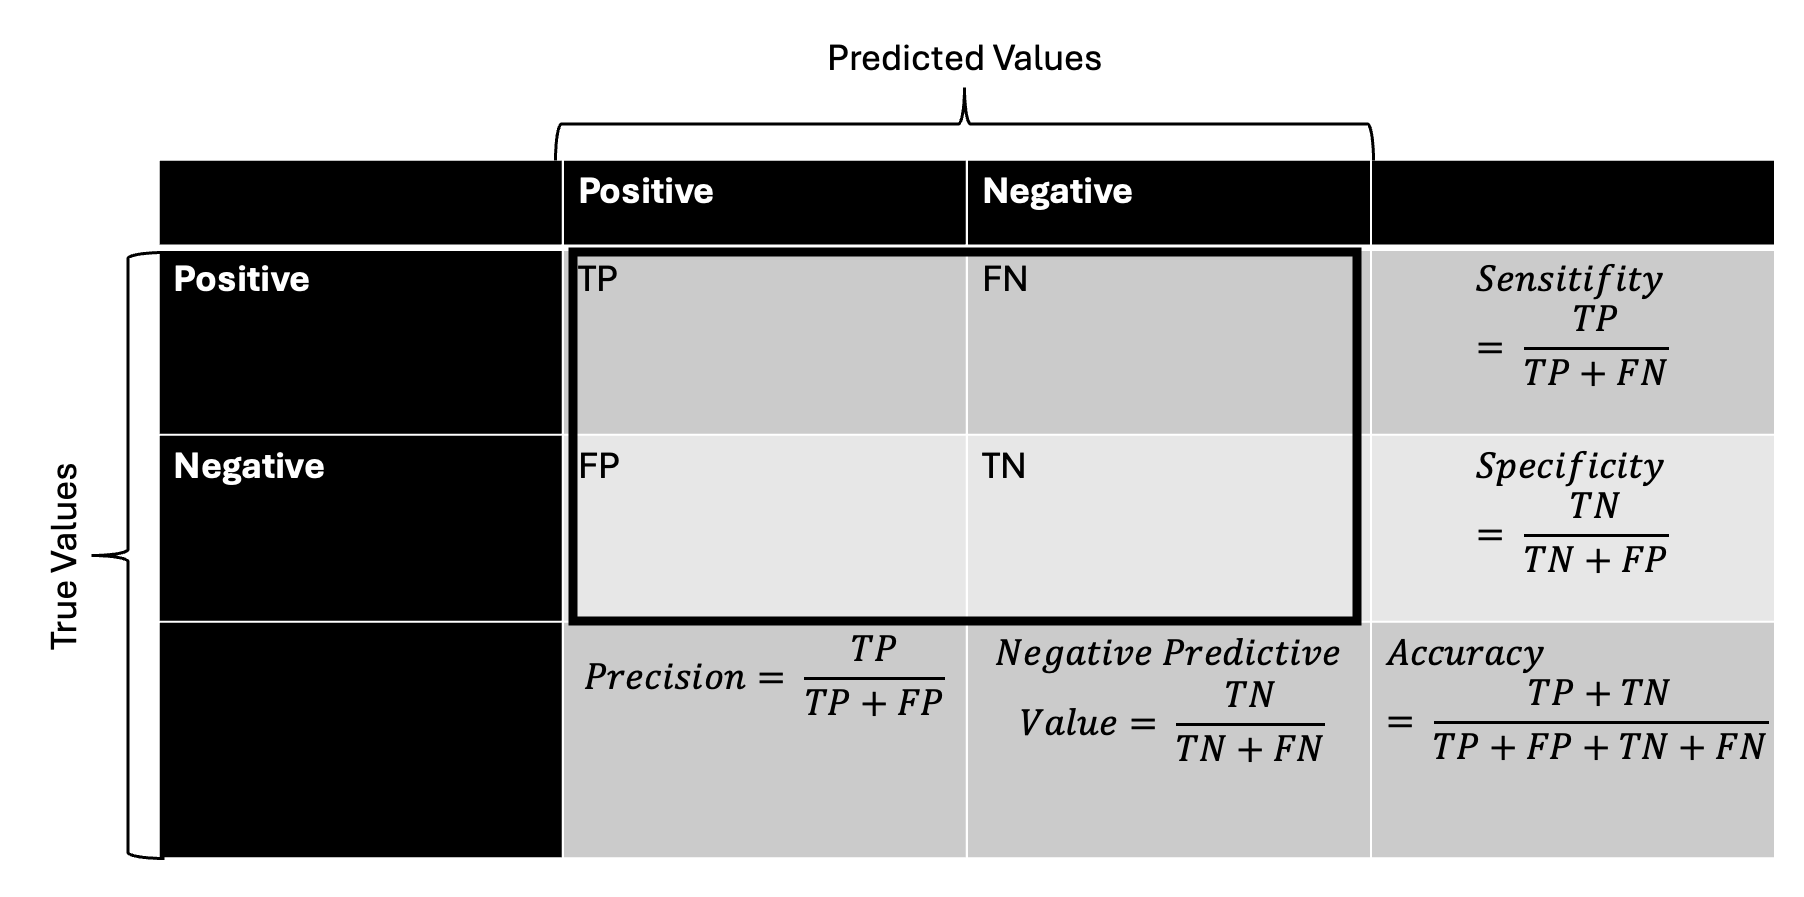
\includegraphics[width = 0.9 \linewidth]{figure_man/ConfusionMatrix.png}
\end{frame}

% in der graphic FPR TPR ergaenzen

\begin{frame}{Calibration}
Consider the true positive $Y=1$, true negative $Y=0$, and predicted label $\hat Y$. 

\smallskip

\textbf{Calibration}: When the predicted probabilities $\hat{p}$ closely agree with the observed proportion for $Y = 1$ (for any reasonable grouping).
\begin{itemize}
    \item<1-> \textbf{Calibration in the large}: Observed vs. predicted prob. in \textit{full sample}.
    \only<1> {\centering\includegraphics[page=3, width=0.75\textwidth]{figure_man/calibration_large_vs_small.pdf}}
    \item<2-> \textbf{Calibration in the small}: Observed vs. predicted prob. in \textit{subsets}.
    
  \only<2> {\centering\includegraphics[page=4, width=0.75\textwidth]{figure_man/calibration_large_vs_small.pdf}}
\end{itemize}
\end{frame}




% \begin{frame}{Calibration versus Discrimination}

% \begin{itemize}
% \setlength\itemsep{1em}
%     \item Calibration indicates the agreement between estimated probabilities and observed class frequencies.
%     \item Discrimination is a model's ability to correctly separate observations into specific groups (depends on the selected threshold).
%     \item Models can over-/underestimate probabilities (poor calibration) and still separate classes (good discrimination) or vice versa.
%       \item Poor calibration occurs with imbalanced classes or when the learner lacks a probabilistic framework (e.g., $k$-NN, trees).
%   % \begin{itemize}
%   %   \item The learner has no probabilistic framework in the first place (e.g.,
%   %   $k$-NN or trees).
%   %   \item Classes are imbalanced.
%   % \end{itemize}
%   \item We distinguish between two different notions of calibration:
%   \begin{itemize}
%     \item \textbf{Calibration in the large} is a property of the 
%     \textit{full} sample.\\
%     $\rightarrow$ Observed class-1 frequency in full sample versus average overall predicted class-1 probability.
%     \item \textbf{Calibration in the small} is a property of \textit{subsets}.\\
%     $\rightarrow$ Observed likelihood in subset versus average predicted class-1 probability in that subset.
%   \end{itemize}
%     % \item Consider a model that predicts a patient's disease risk, where a patient is classified as a high-risk patient if disease risk exceeds 20\%. Patient A has a true risk of 5\% while patient B has a true risk of 30\%. The model predicts roughly the same risk with 19\% for A and 21\% for B. It is poorly calibrated but still separates both patients accurately into low-risk and high-risk groups (good discrimination).
    
% \end{itemize}

% \end{frame}

% \begin{frame}{Calibration in the Large}
%     % https://docs.google.com/presentation/d/1Drnq0Av_5KLfnwbRLnp-Tklgxc93C7BT_UXRCydtoes/edit#slide=id.p
    
%     %Compares observed probability (e.g. proportion of positive instances) with the average predicted probability in the \textit{full sample}.
%     \includegraphics[page=3, width=0.6\textwidth]{figure_man/calibration_large_vs_small.pdf}
%     \includegraphics[page=4, width=0.6\textwidth]{figure_man/calibration_large_vs_small.pdf}
% \end{frame}

% \begin{frame}{Calibration in the Small}
%     Compares observed proportion of positive instances  with the average predicted probability in each subset (often constructed by deciles).
%     \makebox[\linewidth]{\includegraphics[page=2, width=\textwidth]{figure/calibration_large_vs_small.pdf}}
% \end{frame}

% \begin{frame}{Why and When Is Calibration Important?}

%     \begin{itemize}
%         \item Reasoning / interpretation of predicted probabilities as actual risks.
%         \item If you are interested in the computed probability reflecting observed frequencies, you need good calibration.
%         %\item Assume a bank decides how much credit to grant to a customer.
%         %\item The bank needs a fairly accurate probability of default for each customer. The higher the default probability, the lower the loan.
%         %\item Given 1000 customers with a 40\% chance of default predicted by a well-calibrated model, we expect to see roughly 400 defaults in this customer group in our data set, etc.
%         %\item Accurate probabilities are necessary to ensure accurate forecasts of gains and losses of the bank.
%         %\item On the macroeconomic level, regulatory requirements demand accurate probabilities in bank models to ensure healthiness of the financial system as a whole.


%    \item \textbf{Example: Medical Diagnosis}

% \begin{itemize}
%     \item In medicine, a well-calibrated model is crucial for decision-making.
%     \item If a diagnostic test predicts 90\% probability of a disease, but only 50\% of patients with that predicted probability have the disease, it's poorly calibrated.
%     \item Poor calibration can lead to misdiagnosis, unnecessary medical procedures, or delayed treatment, impacting patient outcomes.
% \end{itemize}
%     \end{itemize}
% \end{frame}


% ------------------------------------------------------------------------------

% \begin{vbframe}{Discrimination}

% \begin{itemize}
%   \item Consider, again, the binary classification case.
%   \item \textbf{Discrimination} is the ability of a classifier to perfectly 
%   separate the population into positive and negative instances.
%   \begin{itemize}
%     \item The classifier is said to discriminate well if predictions differ 
%     strongly across classes -- e.g., predicted probabilities for the negative 
%     (positive) class are all close to zero (one).
%     \item Measures of discrimination: e.g., AUC, sensitivity, specificity.
%   \end{itemize}
% \end{itemize}

% \begin{center}
%   \includegraphics[width = 0.7\textwidth]{figure_man/placeholder_discrimination}
% \end{center}

% \end{vbframe}

% ------------------------------------------------------------------------------

% \begin{frame}{Calibration}

% \begin{itemize}
%   \item 
%   % \textbf{Calibration}, on the other hand, assesses the concordance of 
%   % predicted probabilities with the observed outcome (for any reasonable
%   % grouping). \\
%   For scoring classifiers, evaluating 
%   calibrations requires transformation of scores to posterior probabilities 
%   first.
%   \item Predictions of a well-calibrated classifier follow approximately the 
%   same distribution as the true data labels.
%   \item Poor calibration occurs with imbalanced classes or when the learner 
%   lacks a probabilistic framework (e.g., $k$-NN, trees).
%   % \begin{itemize}
%   %   \item The learner has no probabilistic framework in the first place (e.g.,
%   %   $k$-NN or trees).
%   %   \item Classes are imbalanced.
%   % \end{itemize}
%   \item We distinguish two different notions of calibration:
%   \begin{itemize}
%     \item \textbf{Calibration in the large} is a property of the 
%     \textit{full} sample.\\
%     $\rightarrow$ Observed class-1 frequency in full sample vs average overall 
%     predicted class-1 probability.
%     \item \textbf{Calibration in the small} is a property of \textit{subsets}.\\
%     $\rightarrow$ Observed likelihood in subset vs average predicted class-1 
%     probability in that subset.
%   \end{itemize}
% \end{itemize}

% We consider data with a binary outcome $y$.
% \begin{itemize}
%   \item \textbf{Calibration:} When the predicted probabilities closely agree
%     with the observed outcome (for any reasonable grouping).
%   \begin{itemize}
%     \item \textbf{Calibration in the large} is a property of the \textit{full sample}.
%     It compares the observed probability in the full sample  (e.g. proportion of observations for which $y=1$)
% <!-- (e.g., 10% if 10 of 100 individuals have the outcome being predicted, e.g. $y=1$) -->
%     with the average predicted probability in the full sample.
%     \item \textbf{Calibration in the small} is a property of \textit{subsets} of the sample.
%     It compares the observed probability in each subset with the average
%     predicted probability in that subset.
%   \end{itemize}
%   \item \textbf{Discrimination:} Ability to perfectly separate the population into $y=0$ and $y=1$.
%     Measures of discrimination are, for example, AUC, sensitivity, specificity.
% \end{itemize}

% \end{frame}

% ------------------------------------------------------------------------------

% \begin{frame}{Example}

% %<!-- http://www.uphs.upenn.edu/dgimhsr/documents/predictionrules.sp12.pdf -->
%  % \begin{table}[]
%  %    \scriptsize
%  %    \centering
%  %    \begin{tabular}{rrrrr}
%  %      \hline
%  %      ID & truth & prediction $f_1$ & prediction $f_2$ & prediction $f_3$ \\
%  %      \hline
%  %      1 & 1 & 0.9 & 0.6 & 0.9 \\
%  %      2 & 1 & 0.9 & 0.6 & 0.9 \\
%  %      3 & 1 & 0.9 & 0.4 & 0.9 \\
%  %      4 & 0 & 0.1 & 0.4 & 0.7 \\
%  %      5 & 0 & 0.1 & 0.4 & 0.7 \\
%  %      6 & 0 & 0.1 & 0.6 & 0.7 \\ \hline
%  %      avg. class-1 prob. & 50\%  & 50\%  & 50\% & 80\% \\
%  %      \hline
%  %    \end{tabular}
%  %  \end{table}
%  \begin{table}[]
%     \scriptsize
%     \centering
%     \begin{tabular}{rrrrr}
%       \hline
%       ID & truth & prediction $f_1$ & prediction $f_2$ \\
%       \hline
%       1 & 1 & 0.67 & 0.99  \\
%       2 & 1 & 0.67 & 0.99  \\
%       3 & 0 & 0.67 & 0.99  \\
%       4 & 1 & 0.33 & 0.01  \\
%       5 & 0 & 0.33 & 0.01  \\
%       6 & 0 & 0.33 & 0.01  \\

%       % avg. class-1 prob. & 50\%  & 50\%  & 50\% & 80\% \\
%       \hline
%     \end{tabular}
%   \end{table}


% \begin{itemize}
%   \item Classifier $f_1$ is both well-calibrated in the large and the small:
%     \begin{itemize}
%         \item For class-1-probabilities of 0.67, the observed relative freq. of class 1 is 0.67. The same holds for class-1-probabilities of 0.33. 
%         \item For a threshold of 0.5, its discriminative power, indicated by its accuracy, is 0.67.
%     \end{itemize}
%   \item Classifier $f_2$ is not well-calibrated but has the same discriminative power:
%     \begin{itemize}
%         \item For observations with class-1-probabilities of 0.99, one would expect a true label of class 1 almost every time.
%         \item Its discriminative power, with an accuracy of 0.67, is the same as for $f_1$.
%         \item $f_2$ is overconfident: its probabilities indicate that $f_2$ is too confident in classifying instances, which is not backed up by its accuracy.
%     \end{itemize}
%   % Both classifiers have identical calibration in the large, 
%   % but $f_1$ has better discriminative power.
%   % \lz
%   % \begin{table}[]
%   %   \centering
%   %   \begin{tabular}{rrrr}
%   %     \small
%   %     \hline
%   %     observation nr. & truth & prediction $f_1$ & prediction $f_2$ \\
%   %     \hline
%   %     1        & 1     & 1           & 0           \\
%   %     2        & 1     & 1           & 1           \\
%   %     3        & 0     & 0           & 1           \\
%   %     4        & 0     & 0           & 0           \\ \hline
%   %     avg. class-1 prob. & 50\%  & 50\%        & 50\%        \\
%   %     \hline
%   %   \end{tabular}
%   % \end{table}

%   % \lz
% % <<eval = FALSE, echo = FALSE>>=
% % truth = c(1,1,0,0,0,0)
% % pred.rule.1 = c(1,1,0,0,0,0)
% % pred.rule.2 = c(0,0,0,0,1,1)
% % kable(data.frame(truth = truth, "pred rule 1" = pred.rule.1, "pred rule 2" = pred.rule.2))
% % @
% % \lz
% %   \item Conversely, $f_1$ and $f_3$ both discriminate well (e.g., setting thresholds at
% %   0.5 and 0.8, respectively), but $f_3$ is poorly calibrated with class 1 being estimated at an 80\% frequency, as opposed to a true frequency of 50\%.
% %   % \lz
%   %   \begin{table}[]
%   %   \footnotesize
%   %   % \centering
%   %   \begin{tabular}{rrrr}
%   %     \hline
%   %     observation nr. & truth & prediction $f_1$ & prediction $f_2$ \\
%   %     \hline
%   %     1 & 1 & 0.97 & 0.66 \\
%   %     2 & 1 & 0.97 & 0.66 \\
%   %     3 & 0 & 0.01 & 0.45 \\
%   %     4 & 0 & 0.01 & 0.45 \\
%   %     5 & 0 & 0.01 & 0.45 \\
%   %     6 & 0 & 0.01 & 0.45 \\
%   %     % 7 & 0 & 0.01 & 0.67 \\
%   %     % 8 & 0 & 0.01 & 0.67 \\ \hline
%   %     avg. class-1 prob. & 25\%  & 25\%  & 75\% \\
%   %     \hline
%   %   \end{tabular}
%   % \end{table}
%   % \begin{table}[]
%   %   \footnotesize
%   %   % \centering
%   %   \begin{tabular}{rrrr}
%   %     \hline
%   %     observation nr. & truth & prediction $f_1$ & prediction $f_2$ \\
%   %     \hline
%   %     1 & 1 & 0.97 & 0.99 \\
%   %     2 & 1 & 0.97 & 0.99 \\
%   %     3 & 0 & 0.01 & 0.67 \\
%   %     4 & 0 & 0.01 & 0.67 \\
%   %     5 & 0 & 0.01 & 0.67 \\
%   %     6 & 0 & 0.01 & 0.67 \\
%   %     7 & 0 & 0.01 & 0.67 \\
%   %     8 & 0 & 0.01 & 0.67 \\ \hline
%   %     avg. class-1 prob. & 25\%  & 25\%  & 75\% \\
%   %     \hline
%   %   \end{tabular}
%   % \end{table}
%   % \begin{table}[]
%   %  \scriptsize
%   % \centering
%   % \begin{tabular}{rrrr}

%   % \hline
%   % observation nr. & truth & prediction $f_1$ & prediction $f_2$ \\
%   % \hline
%   % 1        & 1     & 0.9           & 0.9         \\
%   % 2        & 1     & 0.9           & 0.9           \\
%   % 3        & 0     & 0.1          & 0.7           \\
%   % 4        & 0     & 0.1         & 0.7           \\ \hline
%   % avg. class-1 prob. & 50\%  & 50\%        & 80\%        \\
%   % \hline
%   % \end{tabular}
%   % \end{table}
%   % \lz
%   % \item Both classifiers discriminate well (e.g., setting thresholds at
%   % 0.5 and 0.8, respectively).
%   % \item Classifier $f_2$ is, however, rather poorly calibrated: the probability 
%   % of class 1 would be estimated at three times the true proportion.
% \end{itemize}
% \end{frame}




\begin{frame}{Calibration and Discrimination}
%<!-- http://www.uphs.upenn.edu/dgimhsr/documents/predictionrules.sp12.pdf -->
A well-calibrated classifier can be poorly discriminating, e.g.

\begin{table}[]
\centering
\begin{tabular}{r|rrr}
\hline
Obs. Nr. & true $Y$ & $\fh_1$ & $\fh_2$ \\
\hline
1        & 1     & 1           & 0           \\
2        & 1     & 1           & 0           \\
3        & 0     & 0           & 1           \\
4        & 0     & 0           & 1           \\ \hline
Avg Prob & 50\%  & 50\%        & 50\%        \\
\hline
\end{tabular}
\end{table}

\begin{itemize}
  \item Both models ($\fh_1$ and $\fh_2$) result in the same calibration in the large (50\%).
  \item However, $\fh_1$ is better than $\fh_2$ as it correctly classifies the real outcome $Y$.
\end{itemize}

\end{frame}

\begin{frame}{Calibration and Discrimination}
A well-discriminating classifier can have a bad calibration, e.g.

\begin{table}[]
\centering
\begin{tabular}{r|rrr}
\hline
Obs. Nr. & truth $Y$ & $\fh_1$ & $\fh_2$ \\
\hline
1        & 1     & 0.7           & 0.9         \\
2        & 1     & 0.7           & 0.9           \\
3        & 0     & 0.3          & 0.5           \\
4        & 0     & 0.3         & 0.5           \\ \hline
Avg Prob & 50\%  & 50\%        & 70\%        \\
\hline
\end{tabular}
\end{table}

\begin{itemize}
  \item Both models are well discriminating, i.e., setting thresholds $c_1 \in ]0.3, 0.7[$ for $\fh_1$ and $c_2 \in ]0.5, 0.9[$ for $\fh_2$ perfectly separates positive and negative observations (and will result, e.g., in a perfect AUC = 1).
  \item $\fh_2$ is poorly calibrated as the averaged probabilities are $70\%$ and do not match the truth proportion of positive observations (which is $50\%$).
\end{itemize}

$\Rightarrow$ \textbf{How can we measure calibration quality?}

\end{frame}

% \begin{frame}{Importance of Calibration}

% % \textbf{Example 1: Weather Forecasting}

% % \begin{itemize}
% %     \item Consider a weather forecasting model that predicts the probability of rain.
% %     \item If the model consistently predicts a 70\% chance of rain, but it actually rains only 10\% of the time when it predicts a 70\% chance, it's poorly calibrated.
% %     \item Poor calibration can lead to bad decisions (carrying an umbrella unnecessarily).
% % \end{itemize}

% \textbf{Example: Medical Diagnosis}

% \begin{itemize}
%     \item In medicine, a well-calibrated model is crucial for decision-making.
%     \item If a diagnostic test predicts 90\% probability of a disease, but only 50\% of patients with that predicted probability have the disease, it's poorly calibrated.
%     \item Poor calibration can lead to misdiagnosis, unnecessary medical procedures, or delayed treatment, impacting patient outcomes.
% \end{itemize}

% \end{frame}








\begin{frame}{Calibration Plot / Reliability Diagram}

%TODO use graphics from paper (equi-width binning): this binning is not so intuitive

%\fbox{
%\parbox[][45pt][t]{\linewidth}
%}

% \begin{columns}[c, onlytextwidth]
%     \begin{column}{0.25\textwidth}
% %\begin{center}
% \centering
% \begin{tabular}{rr}
% \hline
% $\hat{p}$ & $y$ \\
% \hline
%  0.1 & 0 \\
%  0.1 & 0 \\
% \hline
%  0.4 & 0 \\
%  0.4 & 1 \\
% \hline
%  0.7 & 0 \\
%  0.7 & 1 \\
%  0.7 & 1 \\
% \hline
%  0.9 & 1 \\
% \hline
% \end{tabular}
% %\end{center}
%  \end{column}
%         \begin{column}{0.75\textwidth}
% %\begin{center}
% \centering
% 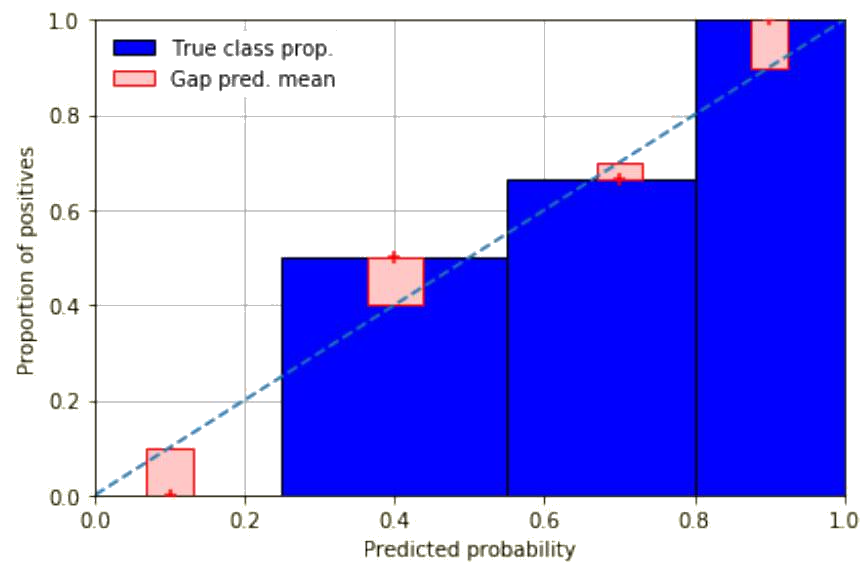
\includegraphics[width=0.85\textwidth]{figure_man/calibplot}
% %\end{center}
%     \end{column}
% \end{columns}

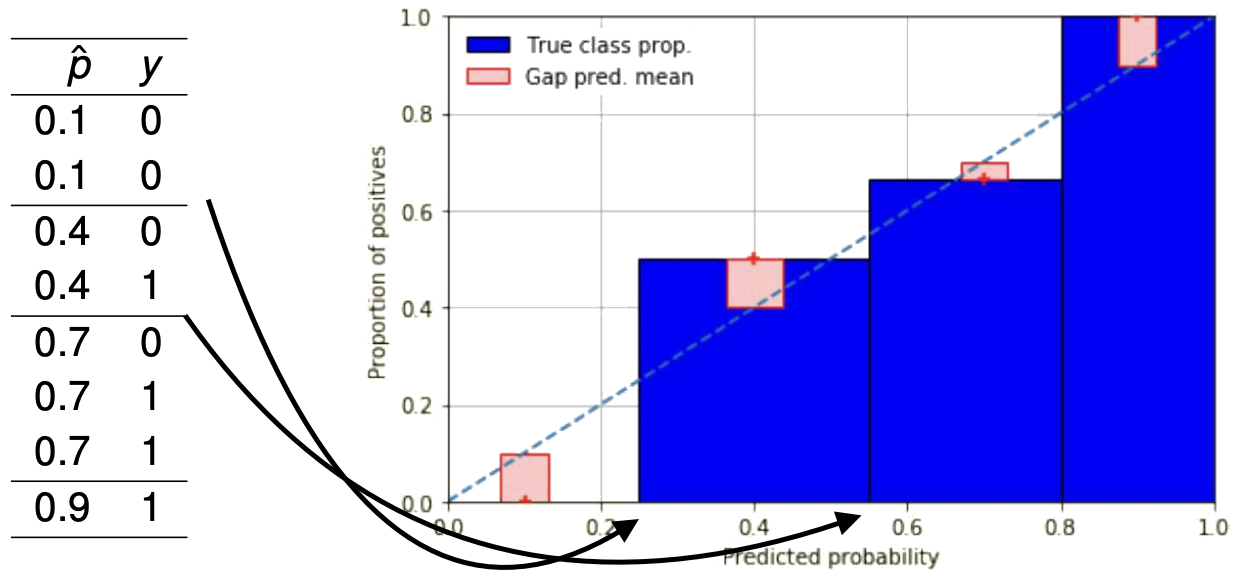
\includegraphics{figure_man/calibplot2.png}

\textbf{Gap pred. mean:} Shows deviation between observed proportion of positives (red points) and average predicted probability within each group (red bar).

\end{frame}



\begin{frame}{Calibration Plot / Reliability Diagram}

%\parbox[][45pt][t]{\linewidth}{%
Changing predictions will change the position of the red points on the x-axis
\begin{itemize}
    \item The closer the red points to the diagonal line, the better calibration
    %\item[$\Rightarrow$] \textit{Gap pred. mean} shows deviation between points and diagonal line
    \item \textbf{Question:} Did we improve or worsen calibration?
\end{itemize}
%}

\begin{columns}[c, onlytextwidth]
    \begin{column}{0.25\textwidth}
%\begin{center}
\centering
\begin{tabular}{rr}
\hline
$\hat{p}$ & $y$ \\
\hline
 0.1 & 0 \\
 \textbf{0.2} & 0 \\
\hline
 \textbf{0.3} & 0 \\
 0.4 & 1 \\
\hline
 \textbf{0.6} & 0 \\
 0.7 & 1 \\
 \textbf{0.8} & 1 \\
\hline
 0.9 & 1 \\
\hline
\end{tabular}
%\end{center}
 \end{column}
        \begin{column}{0.75\textwidth}
%\begin{center}
\centering
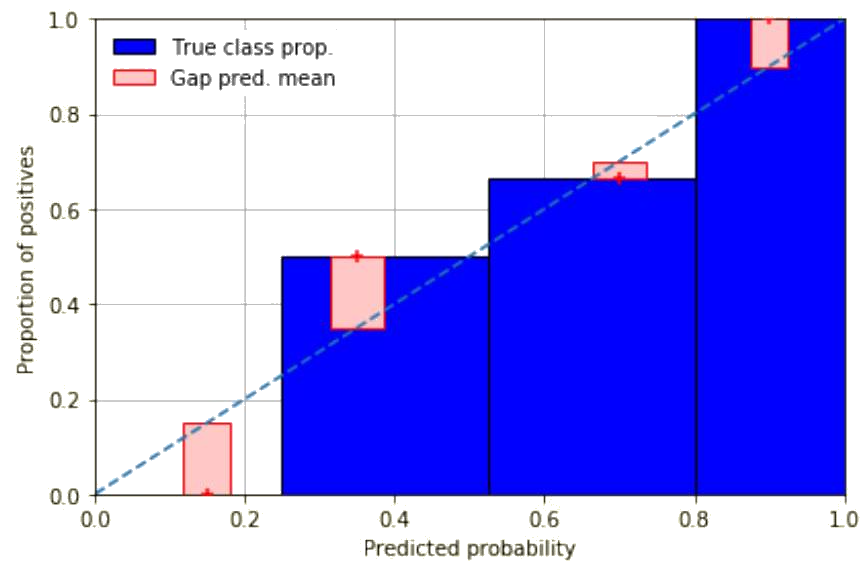
\includegraphics[width=0.85\textwidth]{figure_man/calibplot-2}
%\end{center}

    \end{column}
\end{columns}

\end{frame}




% Frame: Or should we group forecasts differently?
\begin{frame}{Calibration Plot / Reliability Diagram}


Different groupings lead to a completely different picture

\begin{center}
    
\begin{columns}[c, onlytextwidth]

    \begin{column}{0.15\textwidth}
    \raggedleft
    2 Groups
    \end{column}
    \begin{column}{0.30\textwidth}

\footnotesize
\centering
\begin{tabular}{r|r}
$\hat{p}$ & $y$ \\
\hline
 0.1 & 0 \\
 0.2 & 0 \\
 0.3 & 0 \\
 0.4 & 1 \\
\hline
 0.6 & 0 \\
 0.7 & 1 \\
 0.8 & 1 \\
 0.9 & 1 
\end{tabular}

 \end{column}
        \begin{column}{0.47\textwidth}
        \raggedright
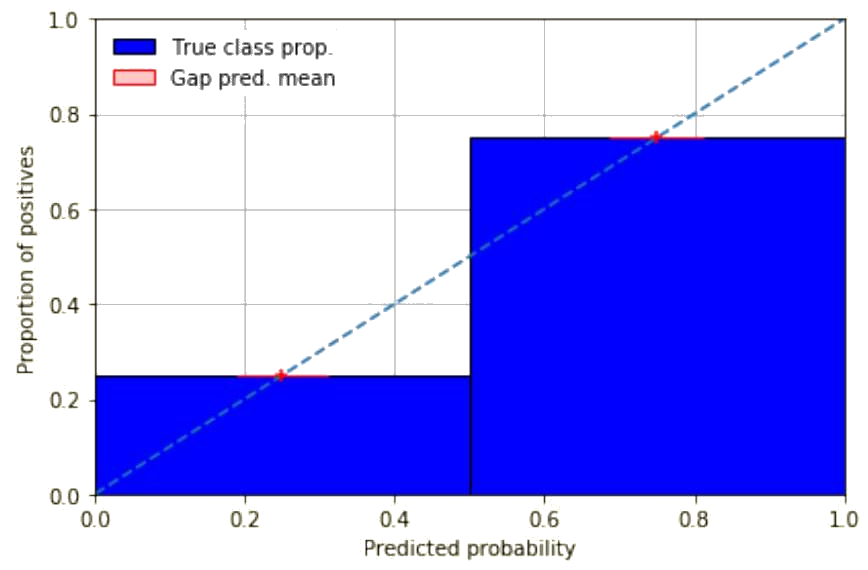
\includegraphics[width=\textwidth]{figure_man/calibplot-3}

    \end{column}
\end{columns}
\pause\hrule
\begin{columns}[c, onlytextwidth]
    \begin{column}{0.15\textwidth}
     \raggedleft 8 Groups
    \end{column}
    \begin{column}{0.30\textwidth}
\footnotesize
\centering
\begin{tabular}{r|r}
$\hat{p}$ & $y$ \\
\hline
 0.1 & 0 \\
\hline
 0.2 & 0 \\
\hline
 0.3 & 0 \\
\hline
 0.4 & 1 \\
\hline
 0.6 & 0 \\
\hline
 0.7 & 1 \\
\hline
 0.8 & 1 \\
\hline
 0.9 & 1 
\end{tabular}

 \end{column}
        \begin{column}{0.47\textwidth}
        \raggedright
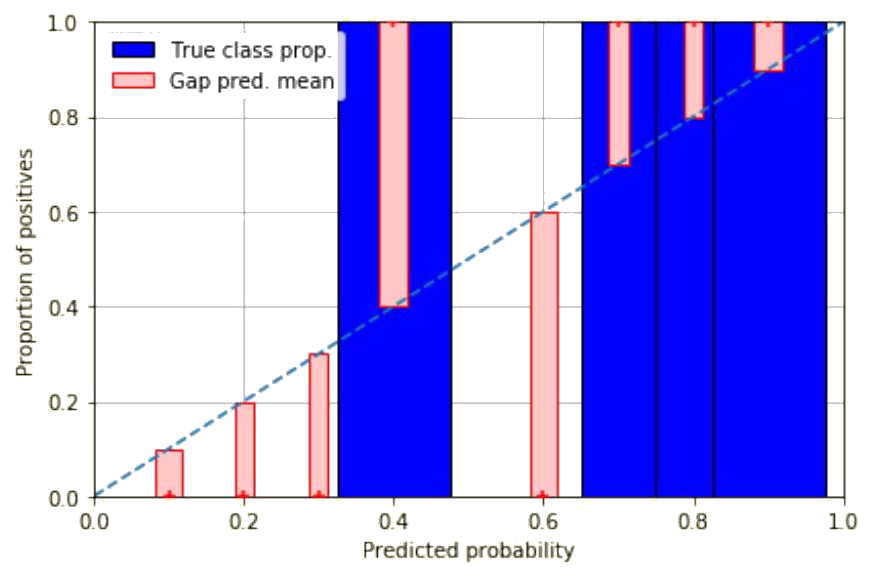
\includegraphics[width=\textwidth]{figure_man/calibplot-4}

    \end{column}    

\end{columns}

\end{center}
\end{frame}

% Frame: Binning or pooling predictions is a fundamental notion
\begin{frame}{Importance of grouping predictions}
\textbf{Evaluating calibration with bins/groups:}
\begin{itemize}
    \item We need enough predictions in each group for reliable estimates.%We need a sufficient number of predictions within each group to obtain reliable empirical estimates.
    \item Trade-off: 
    \begin{itemize}
        \item large groups give better empirical estimates
        \item small groups allow a more fine-grained assessment of calibration
    \end{itemize}
\end{itemize}
% But adjusting forecasts in groups also gives rise to practical calibration methods:
% \begin{itemize}
%     \item empirical binning
%     \item isotonic regression (aka ROC convex hull)
% \end{itemize}
\pause 
\textbf{How groups/bins can be created:}
\begin{itemize}
\item Equal-Width: Splits predicted probabilities into equally sized intervals.\\
$\Rightarrow$ Can lead to bins with few or no observations.
\item Equal-Frequency: Each bin holds a similar number of observations.\\
$\Rightarrow$ Bin width can vary notably.%; Issues with duplicated values.
% \item Empirical Binning: Uses unique values to create bins containing at least a desired number of observations.\\
% $\Rightarrow$ Bin width and bin size may vary; Useful with duplicated values.% similar to equal-frequency in case of no duplicates.
\end{itemize}
\end{frame}




\begin{frame}{ROC Curve vs. Calibration Plot}


{\centering 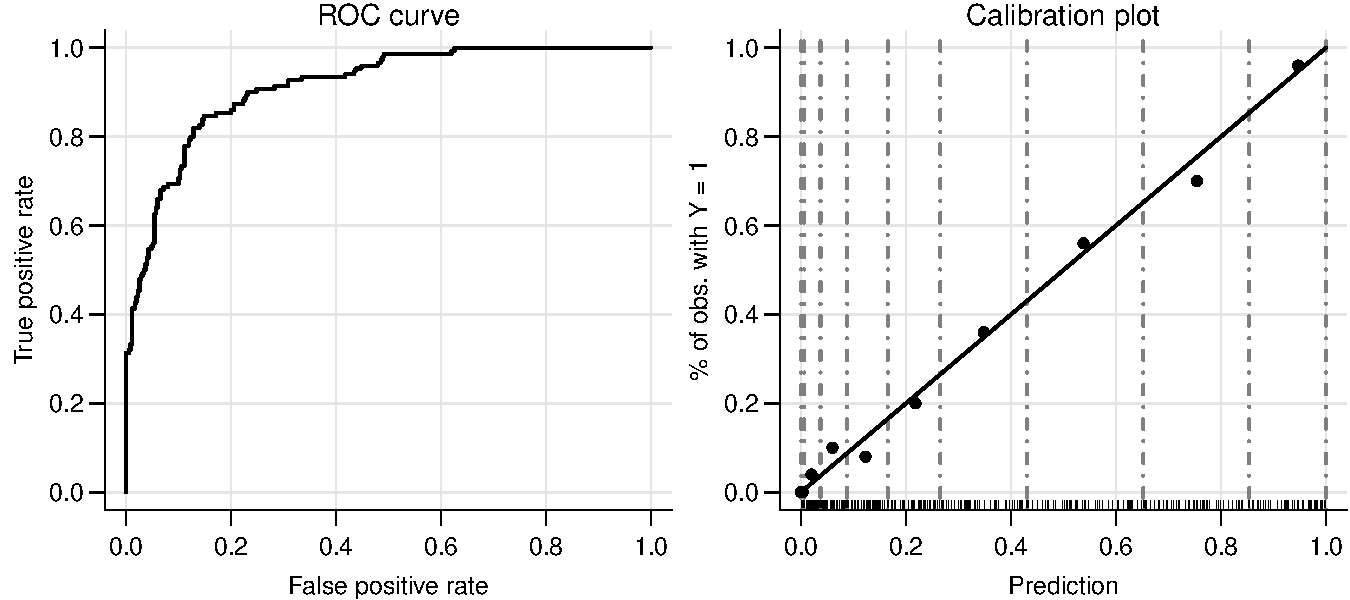
\includegraphics[width=\textwidth]{figure_man/calibdiscr1}}

% and do not visualize how well-calibrated the probabilities are.
%To assess the performance of classifiers, we should consider:
\begin{itemize}
\item \textbf{ROC:}
Measures only discrimination as it is based on TPR and FPR and assesses only the ranking of predicted probabilities (not their magnitude).
%Measures the ability to separate the classes well. % (e.g., confusion matrix). %accurately rank individuals from low to high risk.
\item \textbf{Calibration plot:} Measures (for reasonable groups, here by deciles) how well the predicted probabilities match the proportion of positives. %(i.e., $Y = 1$).
\end{itemize}

\end{frame}


\begin{frame}{ROC Curve vs. Calibration Plot}

{\centering 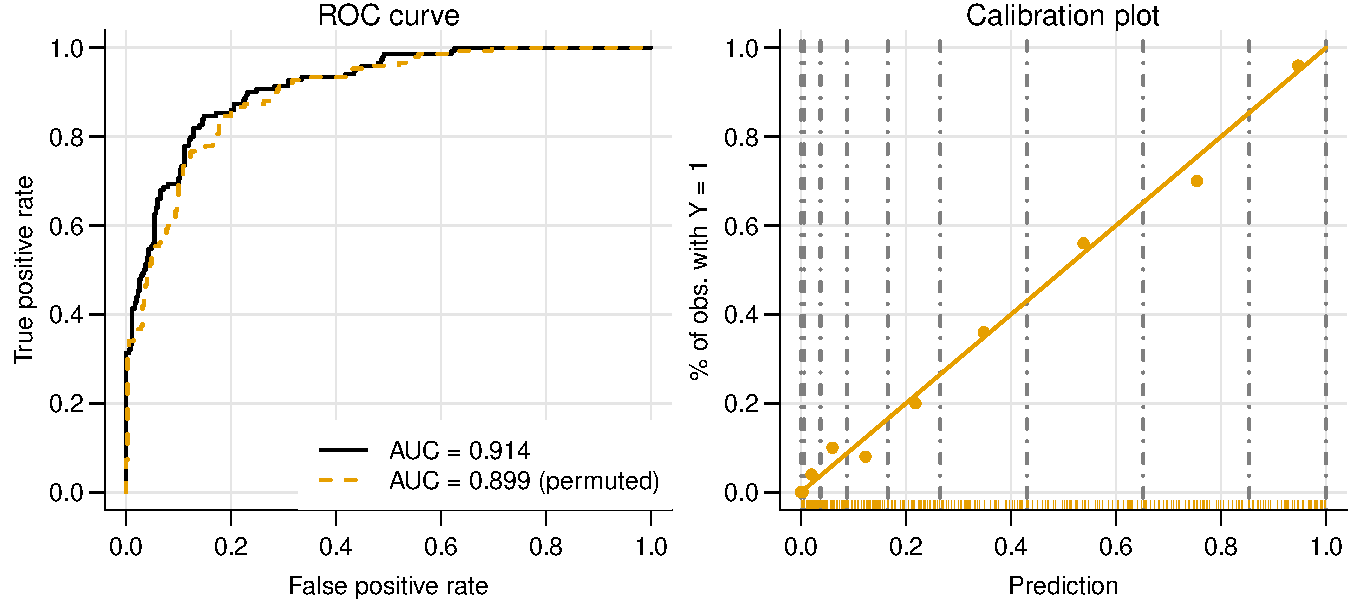
\includegraphics[width=\textwidth]{figure_man/calibdiscr2}}

\vspace{0.5em}

Permuting predictions within each group (e.g., randomly assigning different predictions to observations within each decile)

\begin{itemize}
\item worsens the ROC curve /  AUC (ranking within each decile changes).
\item does not affect the calibration plot (as we only look at averages).
\end{itemize}


\end{frame}


\begin{frame}{ROC Curve vs. Calibration Plot}

{\centering 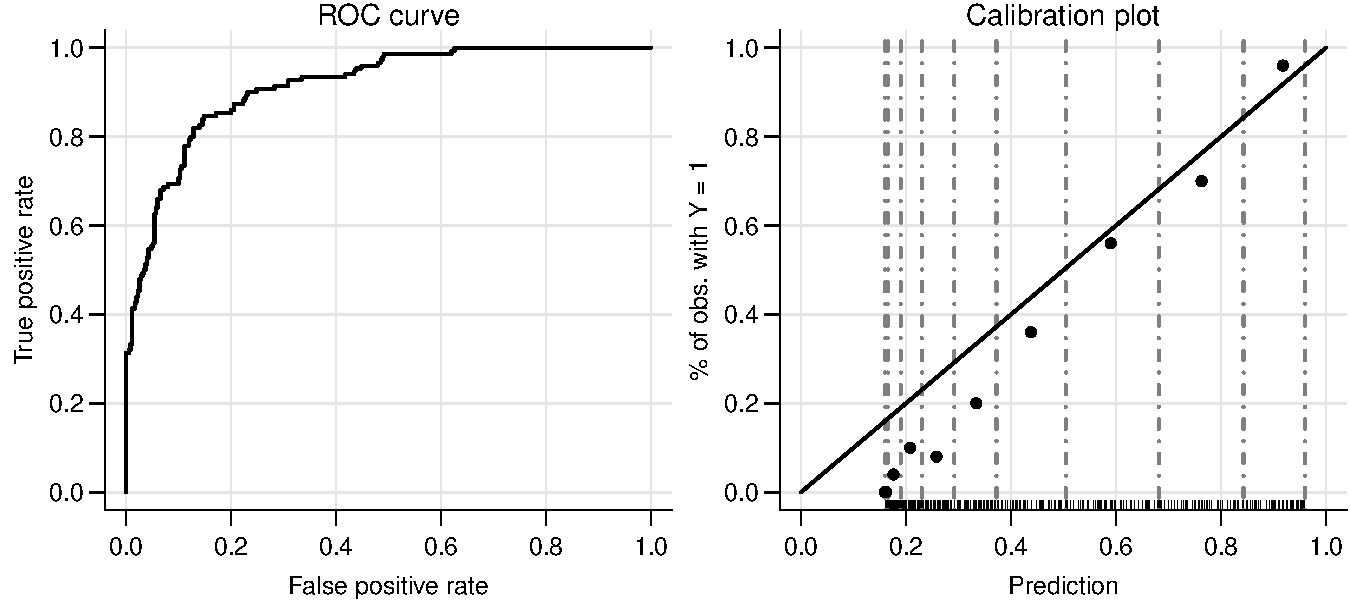
\includegraphics[width=\textwidth]{figure_man/calibdiscr3}}

\vspace{0.5em}

Monotonic transformations of the predicted probabilities (e.g., $\tfrac{\hat p + 0.2}{1.2}$)
\begin{itemize}
\item do not affect the ROC curve as the ranking of $\hat p$ will not change.
\item affect the calibration plot (here it looks worse). %as the probabilities are changed.
\end{itemize}
\end{frame}







% \begin{frame}{Calibration Plots}

% \begin{columns}[c, onlytextwidth]
%     \begin{column}{0.61\linewidth}
% 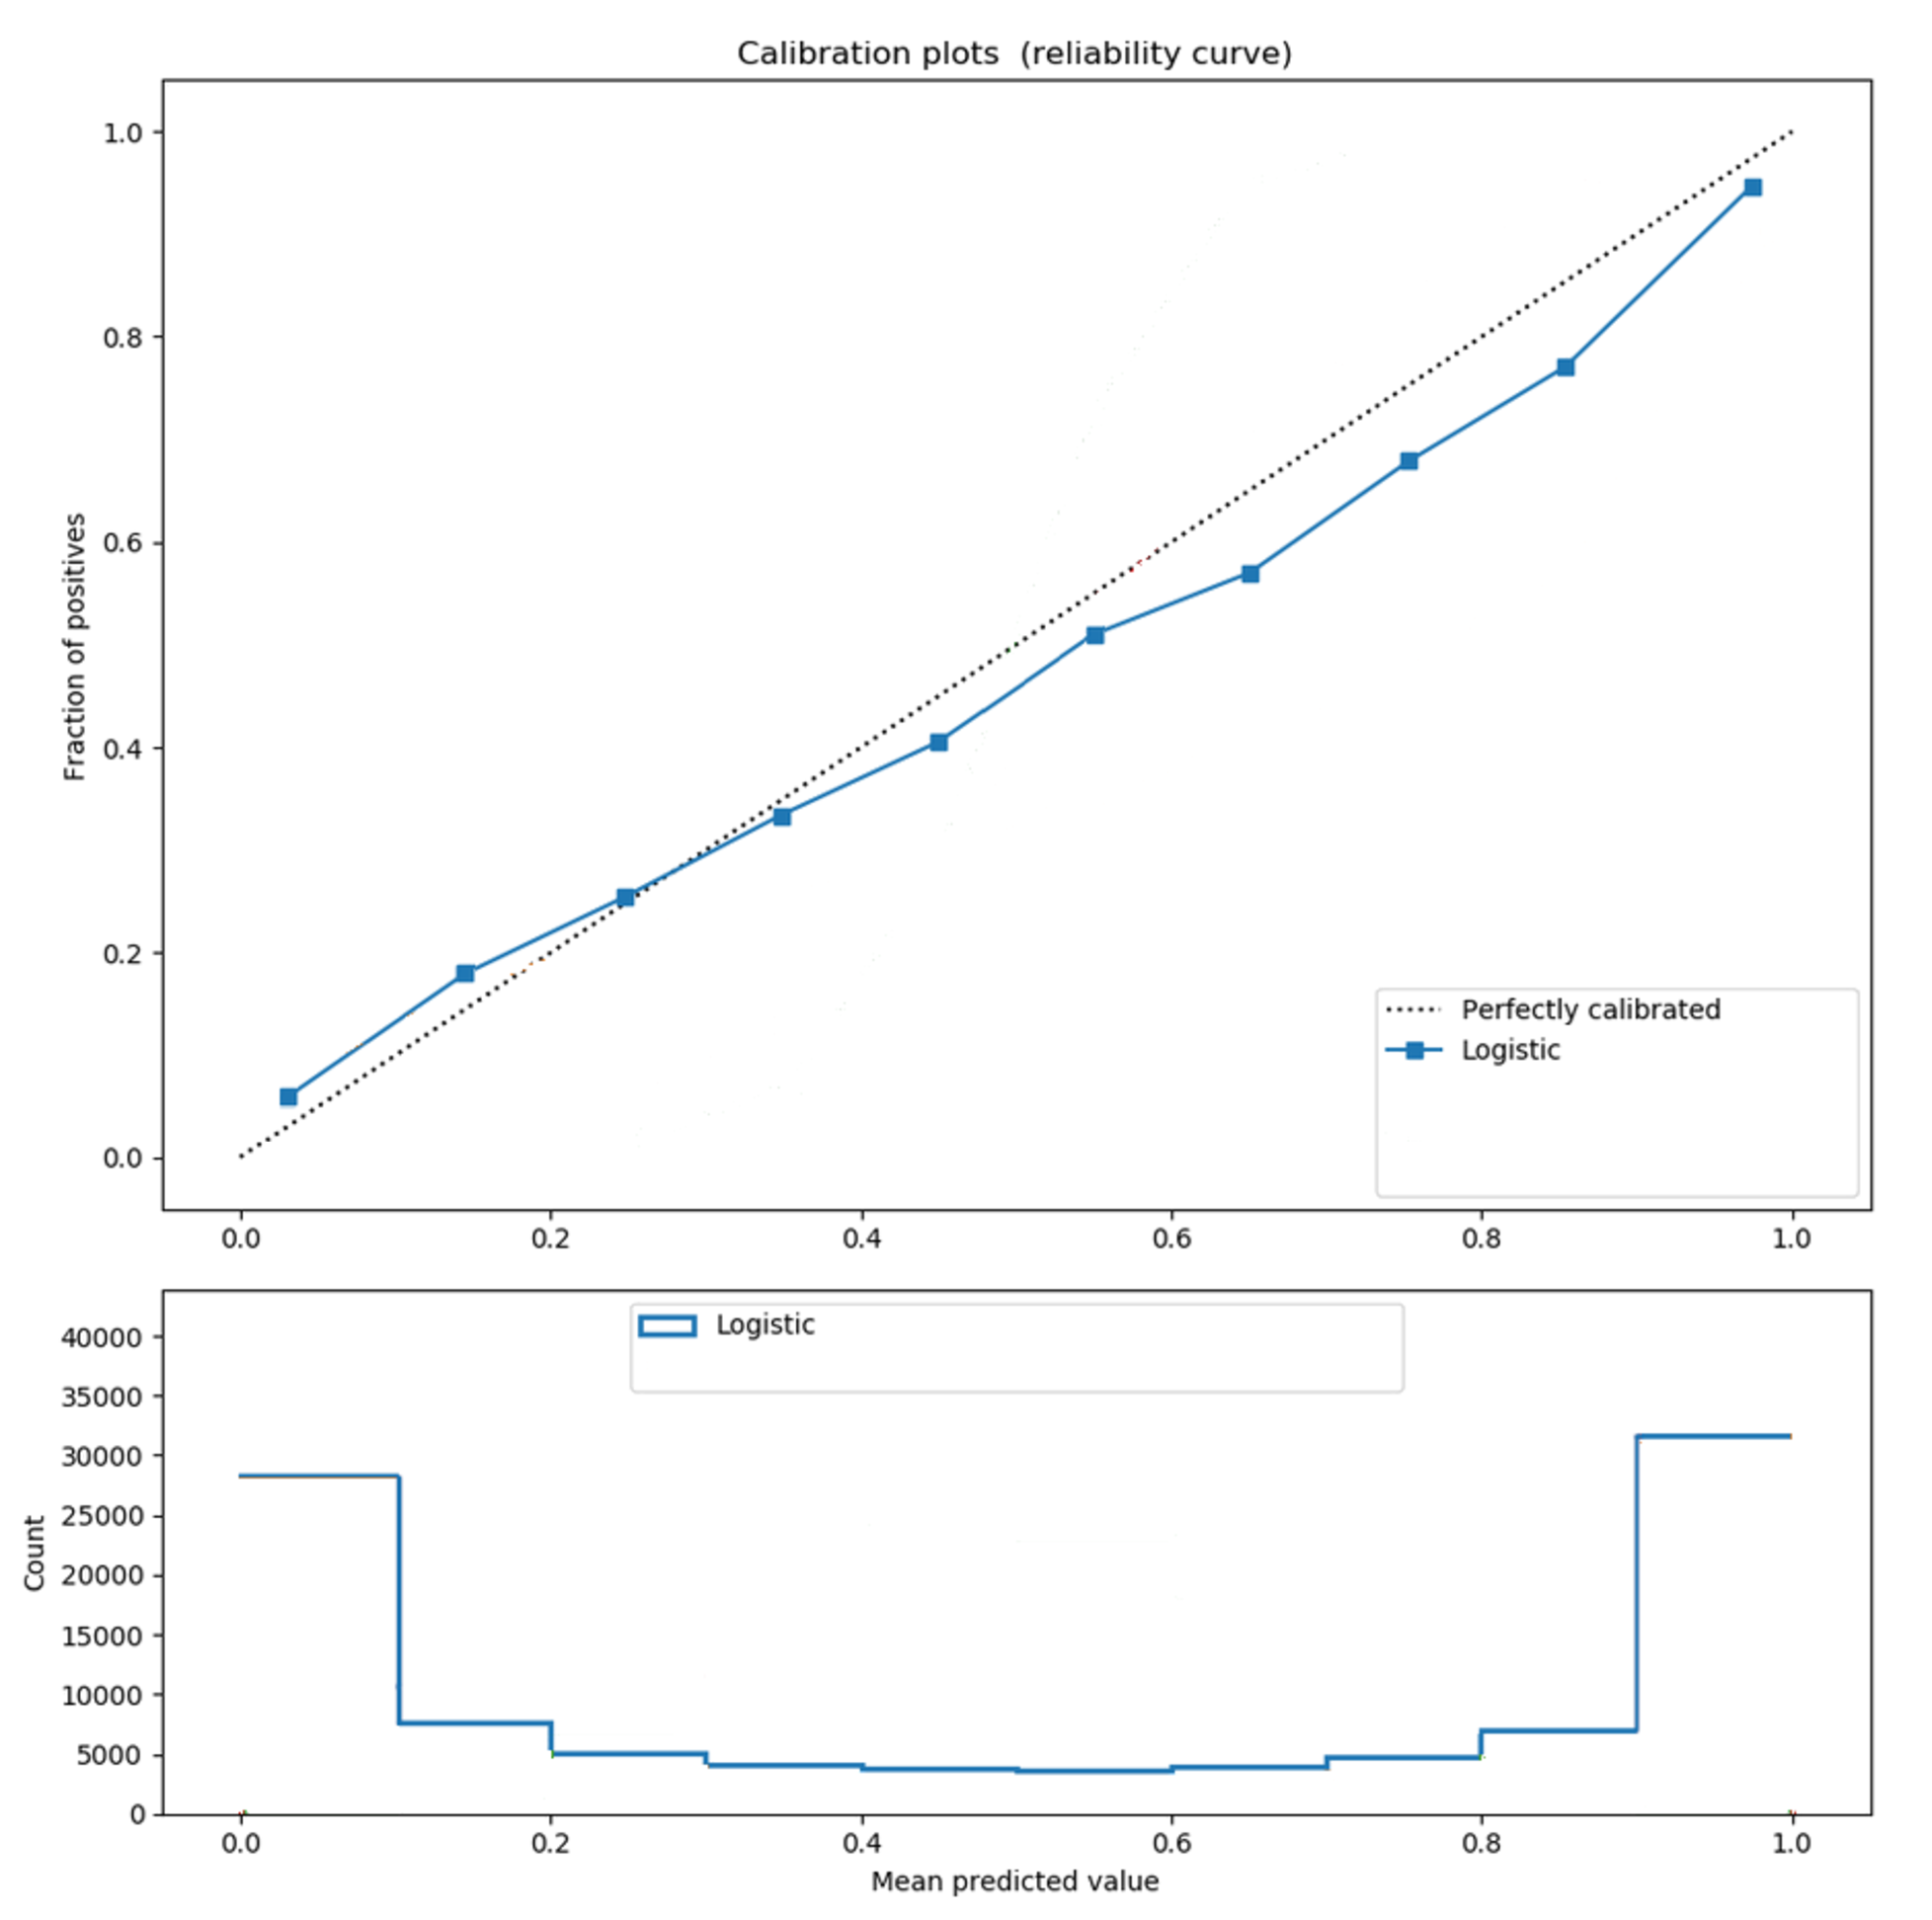
\includegraphics[width=\textwidth, page=1]{figure_man/calibration.pdf}
%     \end{column}
%       \begin{column}{0.39\linewidth}
        
% Calibration plots (reliability diagrams) visualize on
% \begin{itemize}
%     \item $x$-axis: average predicted probability (e.g., grouped by quantiles) 
%     \item $y$-axis: observed proportion of positive instances in each group
% \end{itemize}

%     \end{column}
% \end{columns}

%\end{frame}

\begin{frame}{Example: Calibration Plots  (equal-width)}


\begin{columns}[c, onlytextwidth]
    \begin{column}{0.61\linewidth}

\only<1>{
\includegraphics[width=\textwidth, page=2]{figure_man/calibration.pdf}}
\only<2>{\includegraphics[width=\textwidth, page=3]{figure_man/calibration.pdf}}
\only<3>{\includegraphics[width=\textwidth, page=4]{figure_man/calibration.pdf}}

    \end{column}
      \begin{column}{0.39\linewidth}

        

\begin{itemize}
 %\item Logistic regression is already well-calibrated as it optimzes log-loss
 \item<1-> Many algorithms (except logistic regression) return biased probabilities.
 \item<1-> Linear SVC: badly calibrated, as predictions refer to a distance (to decision boundary) and not to probabilities.
 \item<2-> Random Forest: probabilities close to 0 or 1 are very rare.
 \item<3-> Naive Bayes: pushes probabilities to 0 or 1 (see histograms).
 %Base-level trees trained with random forests incorporate relatively high variance due to feature subsisting
 %(Niculescu-Mizil and Caruana 2005).

\end{itemize}
    \end{column}
\end{columns}

\end{frame}

%TODO include proper scoring rules here (i.e. measure calibration quality)

% \begin{frame}{Metrics for Calibration}

% \textbf{Motivation}: Quantify Calibration Quality

% Let $y$ be the true outcome, $p$ the model's predicted probability, $M$ number of bins, $N$ number of instances

% There is ways to measure ONLY calibration quality:

% \begin{itemize}
%     \item \textbf{Binary estimated calibration error}: average gap across all bins in a reliability diagram, weighted by the number of instances in each bin

%     $$ECE_{binary} = \sum_{m=1}^M \frac{|B_m|}{N}|\bar{y}(B_m)-\bar{p}(B_m)|$$
%     \item \textbf{Binary maximum calibration error}: maximum gap across all bins in a reliability diagram, weighted by the number of instances in each bin

%     $$MCE_{binary} = \max|\bar{y}(B_m)-\bar{p}(B_m)|$$

    
% \end{itemize}
    
% \end{frame}


% \begin{frame}{Metrics for Calibration}
% \textbf{Goal}: Assess alignment between predicted probabilities and observed outcomes

% \medskip
% We assume:
% \begin{itemize}
%     \item $y_i \in \{0, 1\}$ true labels, $p_i \in [0,1]$ predicted probabilities
%     \item $B_m$ denotes the $m$-th bin of predicted probabilities
% \end{itemize}

% \medskip
% \textbf{Calibration-only Metrics}:
% \begin{itemize}
%     \item \textbf{Expected Calibration Error (ECE)}: Average absolute deviation between accuracy and confidence
%     \[
%     \mathrm{ECE} = \sum_{m=1}^M \frac{|B_m|}{N} \left| \bar{y}(B_m) - \bar{p}(B_m) \right|
%     \]
    
%     \item \textbf{Maximum Calibration Error (MCE)}: Worst-case deviation across all bins
%     \[
%     \mathrm{MCE} = \max_{m \in \{1, \dots, M\}} \left| \bar{y}(B_m) - \bar{p}(B_m) \right|
%     \]
% \end{itemize}
% \end{frame}
\begin{frame}{Metrics for Calibration}
\textbf{Goal}: Measure agreement between pred. probabilities and observed freq.

%\medskip
%Assume:
\begin{itemize}
    \item $N$ instances; $\hat p \in [0,1]$ predicted probabilities; $y \in \{0,1\}$ true labels
    \item Predictions are grouped into $M$ disjoint bins $B_1, \dots, B_M$
    \item $\bar{p}_m$: average predicted probability in bin $B_m$
    \item $\bar{y}_m$: average true label in bin $B_m$
\end{itemize}

%\medskip
\textbf{Calibration-only Metrics}: Measure how well predicted probabilities match observed frequencies, independent of class separation.
\begin{columns}[c, onlytextwidth]
    \begin{column}{0.6\textwidth}
        \begin{itemize}
    \item \textbf{Expected Calibration Error (ECE)}: Average bin-wise gap between predicted probabilities and actual frequencies $\textstyle \mathrm{ECE} = \sum_{m=1}^M \frac{|B_m|}{N} \left| \bar{y}_m - \bar{p}_m \right|$

    \item \textbf{Maximum Calibration Error (MCE)}: Largest bin-wise gap between predicted probabilities and actual frequencies $\mathrm{MCE} = \max_{1 \leq m \leq M} \left| \bar{y}_m - \bar{p}_m \right|$
\end{itemize}
    \end{column}
    \begin{column}{0.4\textwidth}
        \centering
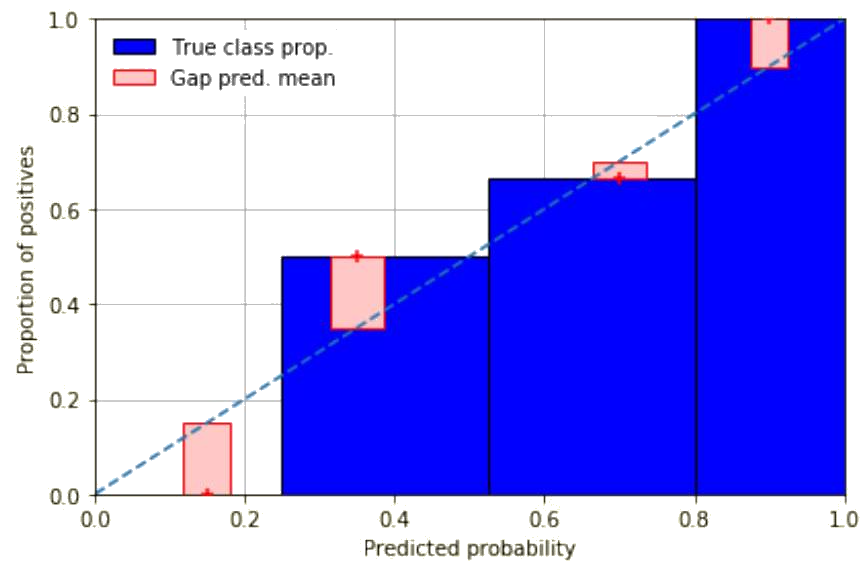
\includegraphics[width=\textwidth]{figure_man/calibplot-2}
    \end{column}
\end{columns}

\end{frame}


\begin{frame}{Hypothesis Test for Calibration}


%\textbf{Approach}:

\begin{itemize}
\item \textbf{Goal}: Test if a classifier is really uncalibrated on the given data set
    \item Group instances into $M$ bins based on percentiles of the predicted probabilities for the
positive class (equal-frequency binning)
\item Compute the test statistics of the Hosmer-Lemeshow (HL) test

$$H = \sum_{m=1}^{M} \left( \frac{(O_m^+ - E_m^+)^2}{E_m^+} + \frac{(O_m^- - E_m^-)^2}{E_m^-} \right)$$

\begin{itemize}
    \item $M$ number of bins
    \item $O_m^+$ observed positives or $O_m^-$ observed negatives in bin $m$
    \item $E_m^+ = N_m \times \bar{p}_m$ expected positives 
    \item $E_m^- = N_m \times (1 - \bar{p}_m)$ expected negatives in bin $m$
    \item $N_m$ number of obs. and $\bar{p}_m$ average predictions in bin $m$
\end{itemize}

\item If $H$ is small $\Rightarrow$ observed outcomes match predicted probabilities (well-calibrated model)

\item Follows a Chi-Squared distribution with $M-2$ degrees of freedom %Calculate p-value on this
\end{itemize}
    
\end{frame}

\begin{frame}{HL Test: Example}

\begin{center}
\footnotesize 
\begin{tabular}{r|rrr}
\hline
Obs. Nr. & truth $Y$ & $\fh_1$ & $\fh_2$ \\
\hline
1 & 1 & 0.9 & 0.9 \\
2 & 1 & 0.9 & 0.9 \\
\hline
3 & 0 & 0.1 & 0.7 \\
4 & 0 & 0.1 & 0.7 \\
\hline
\end{tabular}
\end{center}

Group obs. by their predicted probability, creating $M=2$ bins for each model.

%\begin{center}
{%\footnotesize % Use a smaller font for the tables to ensure they fit
\begin{columns}[T, onlytextwidth]
    \begin{column}{0.5\textwidth}
    \centering
        \textbf{Model $\fh_1$ (Well-calibrated)}
                \begin{tabular}{@{}c|cc|cc@{}}
\hline
            Bin ($\hat{p}$) & $O^+$ & $E^+$ & $O^-$ & $E^-$ \\
\hline
            0.9 & 2 & 1.8 & 0 & 0.2 \\
            0.1 & 0 & 0.2 & 2 & 1.8 \\
\hline
        \end{tabular}
        \begin{align*}
H =& \left( \tfrac{(0-0.2)^2}{0.2} + \tfrac{(2-1.8)^2}{1.8} \right) + \\ &\left( \tfrac{(2-1.8)^2}{1.8} + \tfrac{(0-0.2)^2}{0.2} \right) = 0.44
\end{align*}

    \end{column}
    \begin{column}{0.5\textwidth}
    \centering
        \textbf{Model $\fh_2$ (Poorly calibrated)}
        %\vspace{0.5em}
        \begin{tabular}{@{}c|cc|cc@{}}
\hline
            Bin ($\hat{p}$) & $O^+$ & $E^+$ & $O^-$ & $E^-$ \\
\hline
            0.9 & 2 & 1.8 & 0 & 0.2 \\
            0.7 & 0 & 1.4 & 2 & 0.6 \\
\hline
        \end{tabular}
                \begin{align*}
H =& \left( \tfrac{(0-1.4)^2}{1.4} + \tfrac{(2-0.6)^2}{0.6} \right) + \\ &\left( \tfrac{(2-1.8)^2}{1.8} + \tfrac{(0-0.2)^2}{0.2} \right) = 4.89
\end{align*}
    \end{column}
\end{columns}
%\end{center}
}
\medskip

\textbf{Conclusion:} H-L statistic for $\fh_2$ is over 10 times larger due to a large discrepancy for the $\hat{p}=0.7$ bin ($O^+=0$ vs. $E^+=1.4$). %drives the high H-value, quantifying its poor calibration.

%\vfill
%\textbf{Conclusion:} The H-L statistic for $\fh_2$ is more than 10x larger than for $\fh_1$. This confirms our earlier intuition: the large gap between observed ($O^+$) and expected ($E^+$) outcomes for $\fh_2$ indicates poor calibration.

\end{frame}

\begin{frame}{Calibration: Over- and Under-estimates}

\textbf{Example:} Weather model predicting daily rain probabilities

\begin{itemize}
    % \item Weather forecasters began considering calibration in the 1950s. % (Brier, 1950).
    % \item Consider a weather forecasting model that predicts the probability of rain.
%     \item If the model consistently predicts a 70\% chance of rain, but it actually rains only 10\% of the time when it predicts a 70\% chance, it's poorly calibrated.
\item Calibration implies: predicted probabilities should (on average) match their observed frequencies \\
    $\Rightarrow$ E.g., `70\% chance of rain' $\rightarrow$ should rain $\approx 70\%$ of the time
    \\
    $\Rightarrow$ Ensures predictions can be interpreted as actual risk/probabilities
    \item Consider the following predictions of a (good performing) classifier:
    
    % \item For all instances where a model predicts a '70\% chance of rain', it should actually have rained $\approx$ 70\% of the time (retrospectively).
    % %\item Applicable to both binary and multi-class classification.
    % \item In general, predicted probabilities for any event happening should (on average) match their observed empirical probabilities.\\
    % $\Rightarrow$ Ensures predictions can be interpreted as actual risk/probabilities.
    % \item Consider the following predictions of a (good performing) classifier:
\end{itemize}
\begin{columns}[c, onlytextwidth]
    \begin{column}{0.15\textwidth}
        \centering
        
\begin{tabular}{rr}
$\hat{p}$ & $y$ \\
\hline
 0.1 & 0 \\
 0.1 & 0 \\
\hline
 0.4 & 0 \\
 0.4 & 1 \\
\hline
 0.7 & 0 \\
 0.7 & 1 \\
 0.7 & 1 \\
\hline
 0.9 & 1 \\
\hline
\end{tabular}
    \end{column}
        \begin{column}{0.85\textwidth}
\begin{itemize}
    \item `10\% chance of rain' was a slight over-estimate ($\bar{y}=0/2=0\%$).
    \item `40\% chance of rain' was a slight under-estimate ($\bar{y}=1/2=50\%$).
    \item `70\% chance of rain' was a slight over-estimate ($\bar{y}=2/3=67\%$).
    \item `90\% chance of rain' was a slight under-estimate ($\bar{y}=1/1=100\%$).
\end{itemize}
    \end{column}
\end{columns}
%\vspace{1em}
%\textbf{Calibration}: Is a post-processing step on predicted probabilities trying to reduce over- and under-estimates.
\end{frame}



\begin{frame}{Calibration: Over- and Under-estimates}
%TODO remove the tabular example and give the graphics from this paper https://link.springer.com/article/10.1007/s10994-023-06336-7

\centerline{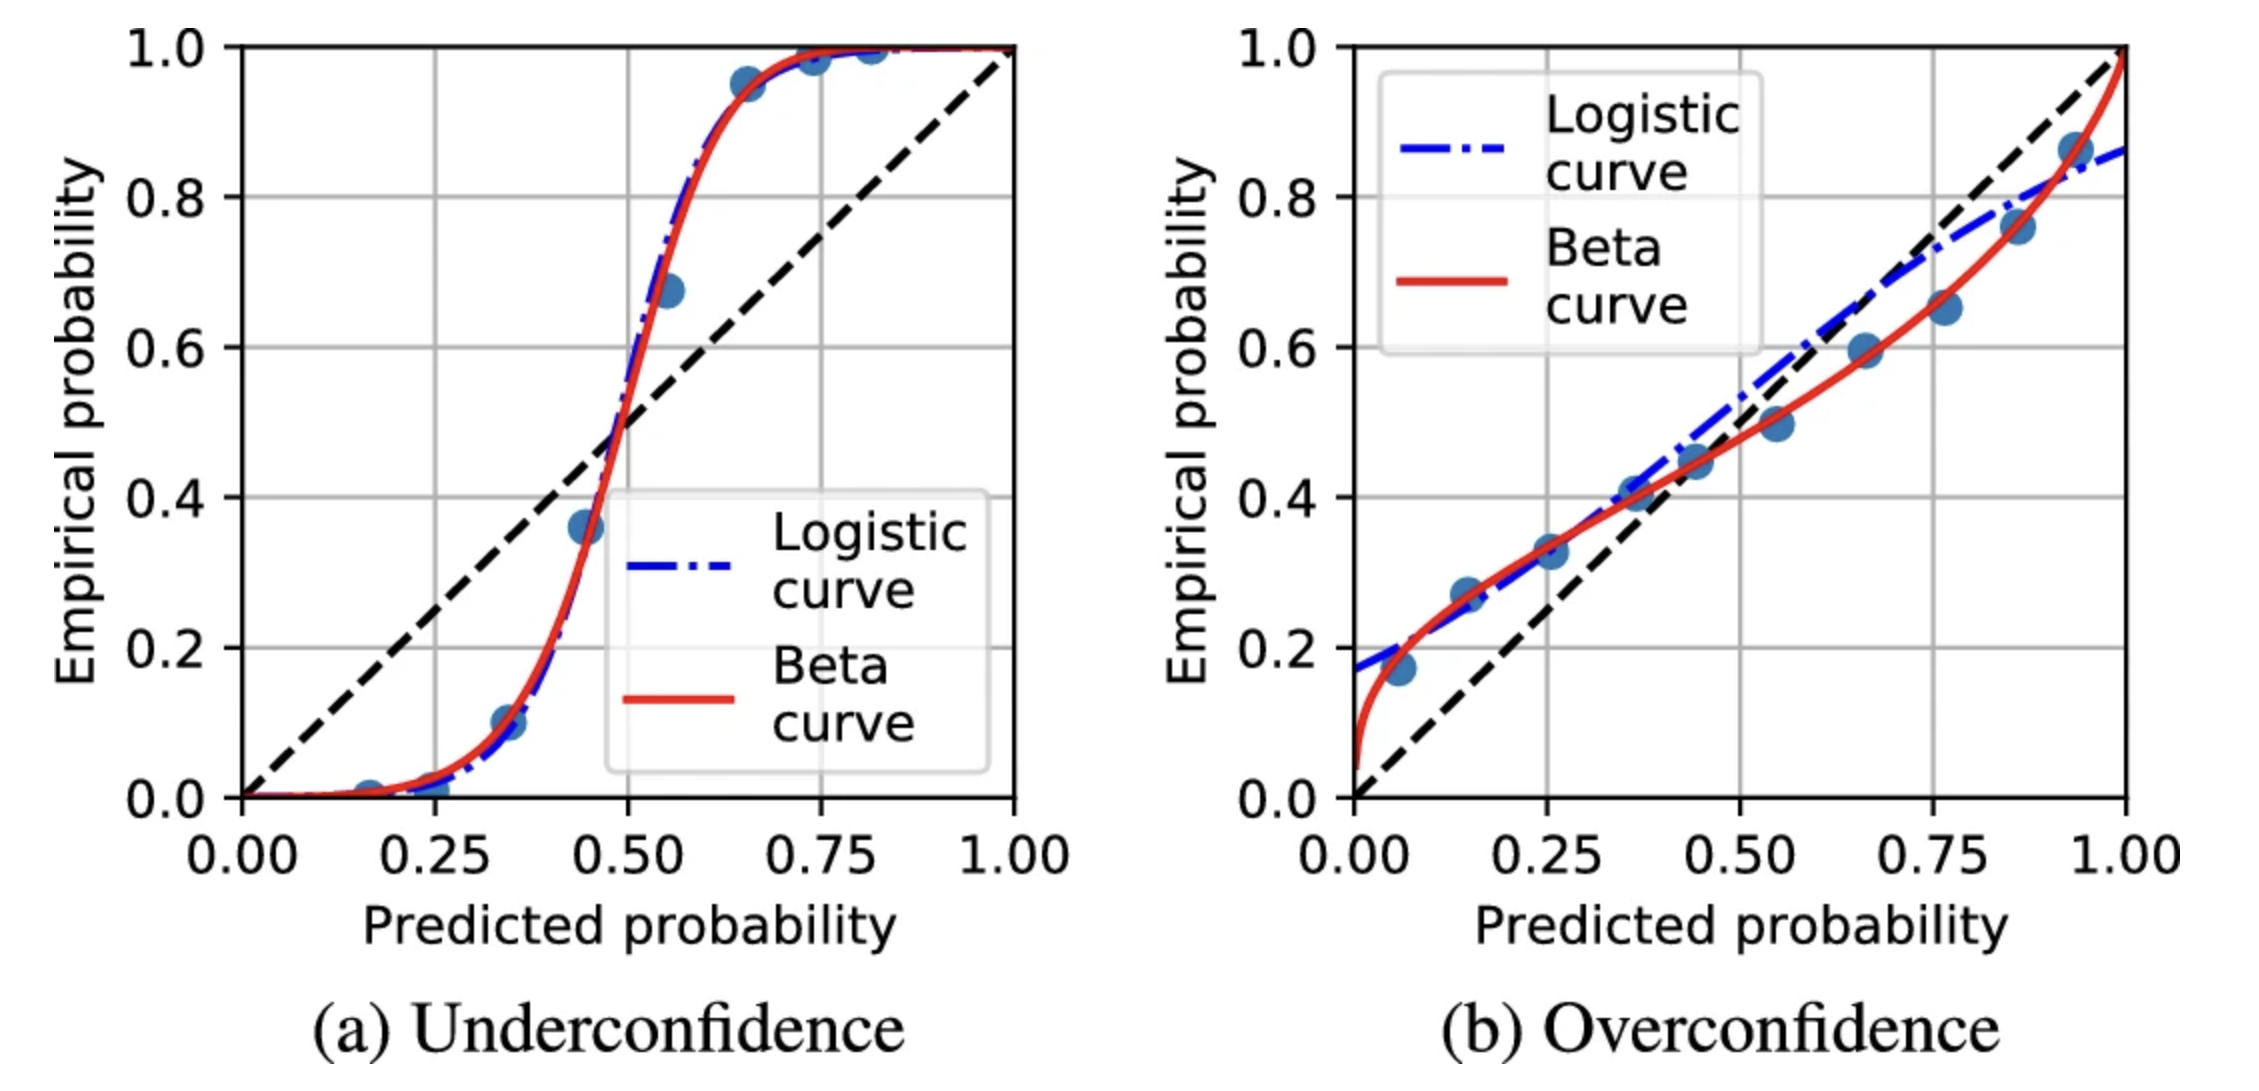
\includegraphics{figure_man/OverAndUnderConfidence.png}}
\centerline{% OLD
%\citebutton{Filho et al. (2023)}{https://link.springer.com/article/10.1007/s10994-023-06336-7/figures/3}
% NEW
\furtherreading{FILHO2023}}

\begin{itemize}
    \item \textbf{Underconfidence}: 
    Predicted probabilities are too close to 0.5 \& need to be expanded (underestimates near 1, overestimates near 0)
    %dots should move outwards on the x-axis (i.e., classifier should be more confident)
    \item \textbf{Overconfidence}: Predicted probabilities are too close to 0 or 1 \&  should be pulled toward 0.5 (overestimates near 1, underestimates near 0)
    %dots should move inwards on the x-axis (i.e,. classifier should be less confident)
\end{itemize}

%\textbf{Example:} Weather forecasting model that predicts the probability of rain.

%\begin{itemize}
    %\item Weather forecasters began considering calibration in the 1950s. % (Brier, 1950).
    %\item Consider a weather forecasting model that predicts the probability of rain.
% %     \item If the model consistently predicts a 70\% chance of rain, but it actually rains only 10\% of the time when it predicts a 70\% chance, it's poorly calibrated.
    %\item For all instances where a model predicts a '70\% chance of rain', it should actually have rained $\approx$ 70\% of the time (retrospectively).
    %\item Applicable to both binary and multi-class classification.
    % \item In general, predicted probabilities for any event happening should (on average) match their observed empirical probabilities.\\
    % $\Rightarrow$ Ensures predictions can be interpreted as actual risk/probabilities.
    %\item Consider the following predictions of a (good performing) classifier:
%\end{itemize}


% \begin{columns}[c, onlytextwidth]
%     \begin{column}{0.3\textwidth}
%         \begin{center}
%         \small
% \begin{tabular}{rr}
% \hline
% $\hat{p}$ & $y$ \\
% \hline
%  0.1 & 0 \\
%  0.1 & 0 \\
% \hline
%  0.4 & 0 \\
%  0.4 & 1 \\
% \hline
%  0.7 & 0 \\
%  0.7 & 1 \\
%  0.7 & 1 \\
% \hline
%  0.9 & 1 \\
% \hline
% \end{tabular}
% \end{center}
%     \end{column}
%         \begin{column}{0.7\textwidth}
% \begin{itemize}
%     \item '10\% chance of rain' was a slight over-estimate ($\bar{y}=0/2=0\%$).
%     \item '40\% chance of rain' was a slight under-estimate ($\bar{y}=1/2=50\%$).
%     \item '70\% chance of rain' was a slight over-estimate ($\bar{y}=2/3=67\%$).
%     \item '90\% chance of rain' was a slight under-estimate ($\bar{y}=1/1=100\%$).
% \end{itemize}
%     \end{column}
% \end{columns}
% %\vspace{1em}
% %\textbf{Calibration}: Is a post-processing step on predicted probabilities trying to reduce over- and under-estimates.
\end{frame}


\endlecture
\end{document}
